\documentclass[a4paper,ngerman, 11pt, DIV11]{scrartcl}
%\documentclass[a4paper,ngerman, 11pt, pagesize]{report}

%% Päambel
\usepackage[T1]{fontenc}
\usepackage[utf8]{inputenc}
\usepackage{babel}

\usepackage{cite}
\usepackage{xcolor}
\newcommand\Diskussionspunkt[1]{\textcolor{red}{#1}}

\usepackage{url}
% keine rote Rahmen um die Links anzeigen
\usepackage[pdfborderstyle={/S/U/W 0}]{hyperref}
%\usepackage{hyperref}

% Grafikpaket laden
\usepackage{graphicx}

% Tabellen
\usepackage{booktabs}
\usepackage{longtable}

% pdf einbinden (A3)
\usepackage{nextpage}
\usepackage{afterpage}
\usepackage{pdfpages}
\usepackage{typearea}
\usepackage{pdfpages}

\usepackage{lscape}


% Quelltext
\usepackage{listings}
 \usepackage{color}
 
 \definecolor{middlegray}{rgb}{0.5,0.5,0.5}
 \definecolor{lightgray}{rgb}{0.8,0.8,0.8}
 \definecolor{orange}{rgb}{0.8,0.3,0.3}
 \definecolor{yac}{rgb}{0.6,0.6,0.1}
 
  \lstset{
   basicstyle=\scriptsize\ttfamily,
   keywordstyle=\bfseries\ttfamily\color{orange},
   stringstyle=\color{green}\ttfamily,
   commentstyle=\color{middlegray}\ttfamily,
   emph={square}, 
   emphstyle=\color{blue}\texttt,
   emph={[2]root,base},
   emphstyle={[2]\color{yac}\texttt},
   showstringspaces=false,
   flexiblecolumns=false,
   tabsize=2,
   numbers=left,
   numberstyle=\tiny,
   numberblanklines=false,
   stepnumber=1,
   numbersep=10pt,
   xleftmargin=15pt
 }


%%  Variablen
\newcommand{\authorName}{Ladina Bilgery \and Thomas Wieling}
\newcommand{\auftraggeber}{Interessengemeinschaft Wetterstation Arbon}
\newcommand{\auftragnehmer}{Interstaatliche Hochschule für Technik NTB}
\newcommand{\projektName}{Multiplattform-fähiges User Interface und Datenmanagement für die Wetterstation Arbon}
\title{\projektName~(Fachmodul)}
\author{\authorName}
\date{\today}

%%  Create a shorter version for tables. DO NOT CHANGE 
\newcommand\addrow[2]{#1 &#2\\ }
\newcommand\addheading[2]{#1 &#2\\ \hline}
\newcommand\tabularhead{\begin{tabular}{lp{13cm}}
\hline
}
\newcommand\addmulrow[2]{ \begin{minipage}[t][][t]{2.5cm}#1\end{minipage}
   &\begin{minipage}[t][][t]{8cm}
    \begin{enumerate} #2   \end{enumerate}
    \end{minipage}\\ }
\newenvironment{usecase}{\tabularhead}
{\hline\end{tabular}}


% damit Bilder im aktuellen Kapitel dargestellt werden
\usepackage{placeins}
\usepackage{geometry}



%%  Beginn Dokument
\begin{document}
\pagenumbering{roman}
\begin{titlepage}
\maketitle
\thispagestyle{empty} 

\begin{verbatim}

\end{verbatim}


  \begin{tabular}[t]{ll}
	Projekt:       & \quad \projektName \\[1.2ex]
	Auftraggeber:  & \quad \auftraggeber\\[1.2ex]
	Auftragnehmer: & \quad \auftragnehmer\\[1.2ex]
  \end{tabular}

\begin{tabular}{|p{3 cm}|p{3 cm}|p{5 cm}|}
\hline
\textbf{Version} & \textbf{Datum} & \textbf{Autor(en)} \\
\hline
\hline
1.0 & 16.11.2017 & \authorName \\
\hline
\end{tabular}
\end{titlepage}

\setcounter{page}{2}
\tableofcontents          
\clearpage
\pagenumbering{arabic}

%%%%%%%%%%%%%%%%%%%%%%%%%%%%%%%%%%%
%%  Einführung
%%%%%%%%%%%%%%%%%%%%%%%%%%%%%%%%%%%
\section*{Einführung ins Thema}

Die Wetterstation Arbon wurde 2005 als Lehrlingsarbeit des Berufsbildungszentrums Arbon auf Initiative der Technischen Gesellschaft Arbon (TGA) aufgebaut und in Betrieb genommen. Sie besteht aus mehreren Wettersensoren und einer Webcam, die auf einer Plattform auf dem See draussen montiert sind. Die Messwerte werden auf der Webseite\footnote{ \url{https://www.wetter-arbon.ch}}  der Wetterstation Arbon angezeigt.

\begin{figure}[h!]
	\centering
	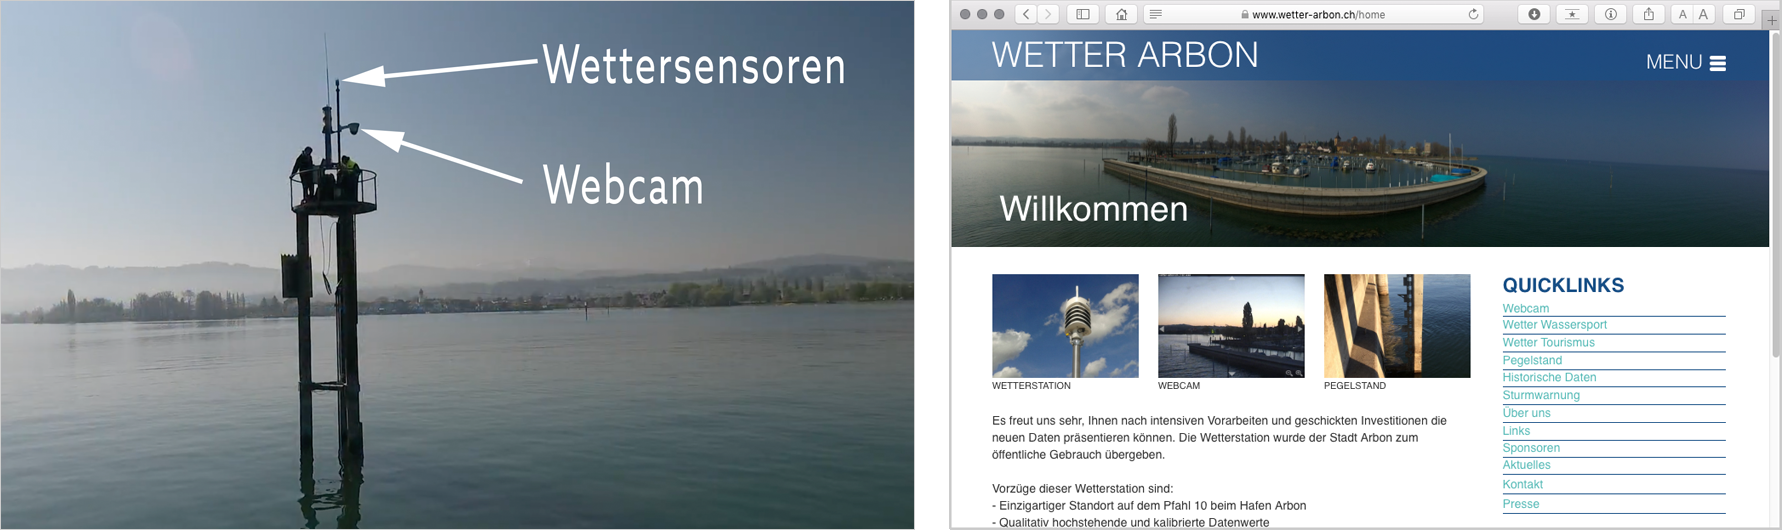
\includegraphics[width=1\linewidth]{img/kombi}
	\caption{Installation und Webseite der Wetterstation Arbon}
	\label{img:wetterstation}
\end{figure}

Was damals modern war, ist heute veraltet. Sowohl auf der Hardwareseite, als auch auf der Webseite gibt es diverses Reparatur- beziehungsweise Modernisierungspotential. Die Bachelor-Arbeit hat das Ziel die Wetterstation wieder auf einen modernen, vollfunktionsfähigen Stand zu bringen. Während des Fachmoduls, welches die Vorbereitung für die Bachelor-Arbeit darstellt, führten wir eine Ist-Aufnahme der Wetterstation Arbon durch. Im Fokus lag sowohl die Hardware als auch die Software. Der Übersicht halber und damit wir die Arbeiten besser untereinander aufteilen konnten, haben wir die Themen in die vier Blöcke:  Webseite, Datenbank, Sensoren und Webcam unterteilt. (vgl. Abb. \ref{img:module})

\vspace{5mm} %5mm vertical space

\begin{figure}[h!]
	\centering
	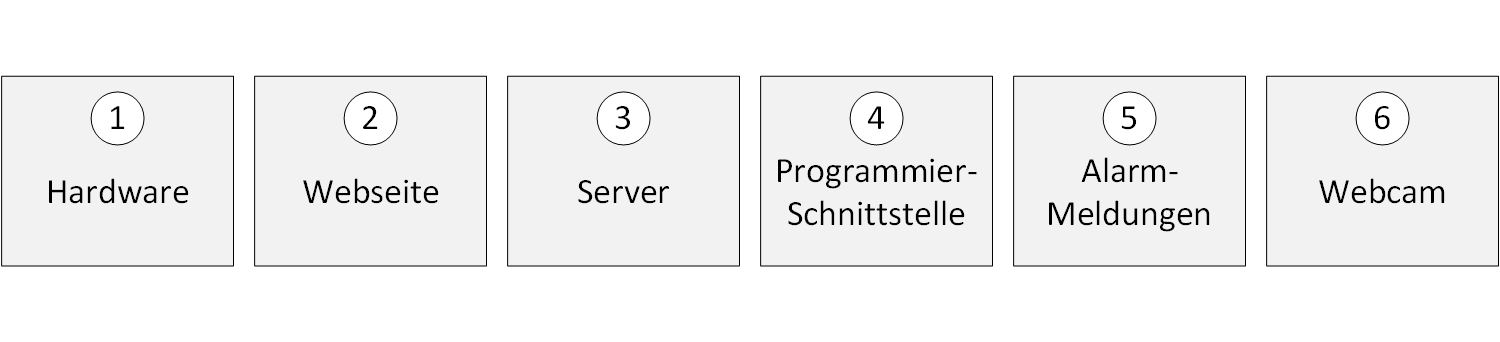
\includegraphics[width=0.8\linewidth]{img/module}
	\caption{Aufteilung in Arbeitsblöcke}
	\label{img:module}
\end{figure}

Dieser Bericht zeigt jeweils pro Block auf, wie die jetzige Situation ist, wo die Problemstellen liegen, wie diese behoben werden können und was die Anforderungen an die Lösung ist. Die Erkenntnisse des Fachmoduls dienen als Grundlage für die Bachelor-Arbeit. Dort geht es darum die Lösungsansätze zu konkretisieren und umzusetzen.

\newpage
%%%%%%%%%%%%%%%%%%%%%%%%%%%%%%%%%%%
%%  Webseite / Front end
%%%%%%%%%%%%%%%%%%%%%%%%%%%%%%%%%%%
\section{Analyse der Webseite (front end)}

Die Webseite der Wetterstation Arbon besteht neben der Homepage aus zwölf Unterseiten. Für uns wichtig sind all jene, die mit den Sensordaten, der Webcam, oder der Datenbank in Verbindung stehen. (hervorgehoben in Abb.\ref{img:sitemap}). Im Folgenden werden die gefundenen Schwachstellen erklärt.

\begin{figure}[h!]
	\centering
	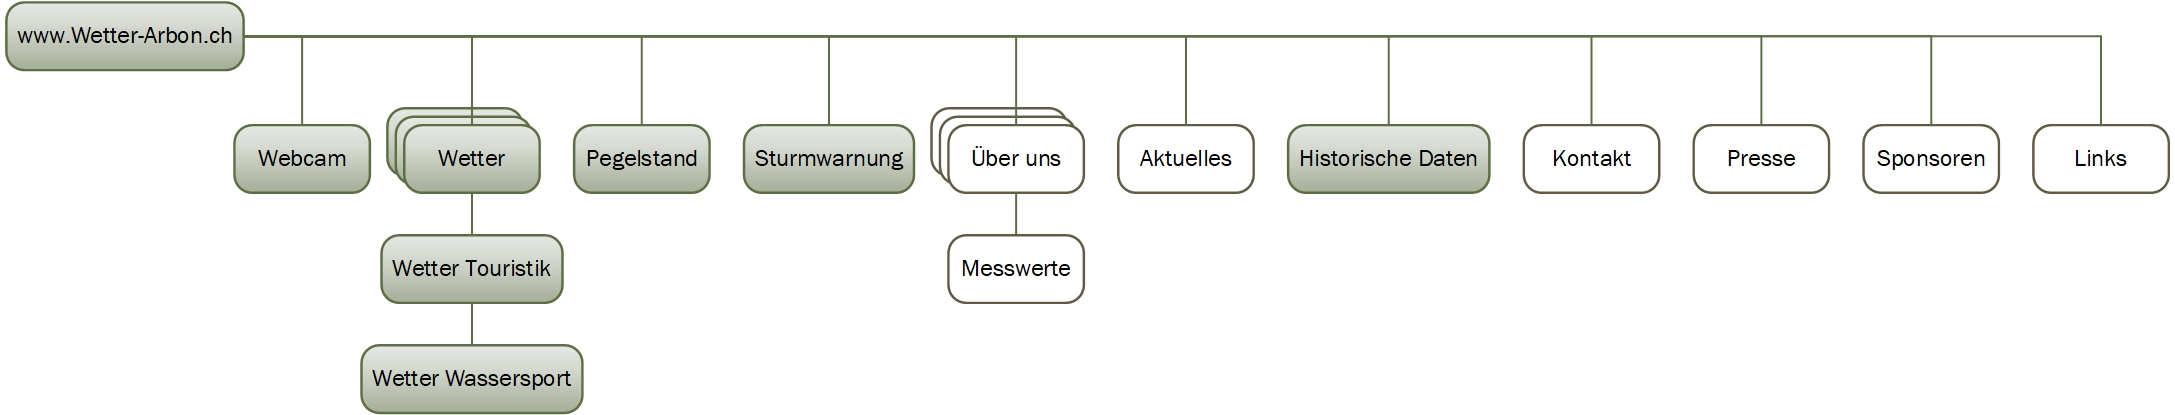
\includegraphics[width=0.9\linewidth]{img/sitemap2}
	\caption{Sitemap der Webseite}
	\label{img:sitemap}
\end{figure}


% #####################################################################################
% Browser-Kompatibilität
% ################################
\subsection{Browser-Kompatibilität}
\label{subsec:flash}
Die Anzeige der Wetterdaten erfolgt durch die Software \textit{WeahterDisplay Live}\footnote{ \url{http://www.weather-display.com/wdlive}}. WeahterDisplay Live erstellt aus den Messwerten eine Adobe Flash Applikation, welche auf der Webseite eingebettet wird, wie in Abbildung~\ref{img:responsive}, dargestellt (gelb markiert).
\newline

\noindent
%\subsection*{Problem}
Adobe Flash war eine einfache Möglichkeit animierte Grafiken auf Webseiten darzustellen und wurde praktisch von allen Browsern, nach Installation des Plug-ins, unterstützt. Diverse Sicherheitslücken und der Umstand, dass es sich um eine proprietäre d.h. closed-source Software handelte, führten dazu, dass Apple 2010 entschied Adobe Flash auf ihrem Mobile-Betiebsystem \textit{iOS} nicht mehr zu unterstützen\cite{Apple:ThoughtsOnFlash}. Sämtliche Adobe Flash Animationen können somit nicht auf iPhone und iPad angezeigt werden.

Da ein Grossteil der Schweizer Bevölkerung jedoch genau diese Mobilgeräte verwendet, wurde für die Wetterstation folgender Workaround geschaffen: Der Browser prüft zuerst, ob das Gerät Adobe Flash unterstützt. Wenn ja wird die normale Applikation geladen, wenn nicht wird ein Printscreen der Applikation geladen. Der Nachteil dieses Workarounds ist jedoch, dass der Printscreen weder dynamisch noch interaktiv ist. Um die aktuellen Werte zu erhalten muss die Seite jeweils neu geladen werden. Die interaktiven Elemente sind unbrauchbar d.h. die Änderung von Einheiten, Anzeige von Rekordwerten und weiteren Graphen ist nicht möglich. Im Juli 2017 hat Adobe zudem angekündigt, dass Adobe Flash im Jahr 2020 eingestellt wird\cite{Adobe:FlashTheFutureofInteractiveContent}.
\newline

\noindent
%\subsection*{Lösungsansatz}
2014 wurde die neue HTML-Spezifikation, HTML5, fertiggestellt. HTML5 bietet diverse neue Funktionen unter anderem im Bereich dynamischer Grafiken. Es ist der neue Web-Standard und wird von allen modernen Web-Browsern unterstützt, ohne dass irgendwelche Plugins installiert werden müssen. Es gibt zudem diverse Javascript-Bibliotheken wie zum Beispiel Google Charts\footnote{ \url{https://developers.google.com/chart/interactive/docs/gallery}} oder D3.js\footnote{ \url{https://github.com/d3/d3/wiki/Gallery}}, mit denen sich ansehnliche und moderne Grafiken erstellen lassen. HTML5 eignet sich somit ideal als Ersatz von Adobe Flash um die Wetterdaten grafisch darzustellen. 


% #####################################################################################
% Barrierefreier Zugang
% ################################
\subsection{Barrierefreier Zugang}
Die Wetterstation und ihre Webseite ist eine Dienstleistung der Stadt Arbon. Sie gehört der Bevölkerung und soll deshalb für möglichst alle zugänglich sein. Sowohl die \flqq Web Content Accessibility Guidelines\frqq\footnote{ \url{https://www.w3.org/TR/2008/REC-WCAG20-20081211/}} des W3C-Konsortiums als auch die deutsche \flqq  Barrierefreie-Informationstechnik-Verordnung\frqq\footnote{ \url{https://www.gesetze-im-internet.de/bitv_2_0/BJNR184300011.html}} bieten diverse Inputs, wie die Bedienbarkeit und somit Zugänglichkeit einer Webseite verbesserte werden kann. 
\newline

\noindent
%\subsection*{Problem}
WeatherDisplay Live, welches zum Anzeigen der Wetterdaten verwendet wird, ist eine proprietäre Software, die nur sehr eingeschränkt angepasst werden kann und auf Adobe Flash basiert. Es lassen sich beispielsweise die Anordnung der Anzeigeelemente und die Einheiten konfigurieren. Viel mehr nicht.  Adobe Flash gilt als kritische Technologie in Hinblick auf Barrierefreiheit. Mit der jetzigen Konfiguration können die Anforderung an eine barrierefreie Seite nicht umgesetzt werde.
\newline

\noindent
%\subsection*{Lösungsansatz}
Wie in Abschnitt \ref{subsec:flash} erläutert, muss WeahterDisplay Live ersetzt werden. Das bietet die Möglichkeit, dass die Entwicklung der neuen Webseite nach den oben erwähnten Richtlinien erfolgen kann.


% #####################################################################################
% Responsive Design
% ################################
\subsection{Responsive Design}
Die Webseite der Wetterstation ist mit dem Content-Management-System (CMS) \textit{Openfile64Light} der Firma Screenbox\footnote{ \url{https://screenbox.net/internet}}  erstellt. Dieses unterstützt grundsätzlich responsive Design. Das CMS gibt den Rahmen der Webseite vor. Spezielle Inhalte wie zum Beispiel die Adobe Flash Animation werden als sogenannte Applikationen behandelt und in die Seite eingebettet, gelb markiert in Abbildung~\ref{img:responsive}, links.
\newline

\noindent
%\subsubsection*{Problem}
Unterstützt die eingebettete Applikation kein responsive Design, so wird dieser Teil einfach linear skaliert. Dies führt dazu, dass die Anzeige der Wetterstationsdaten auf einem Mobilgerät kaum mehr lesbar sind, wie in Abbildung~\ref{img:responsive}, rechts dargestellt.
\newline

\begin{figure}[h!]
	\centering
	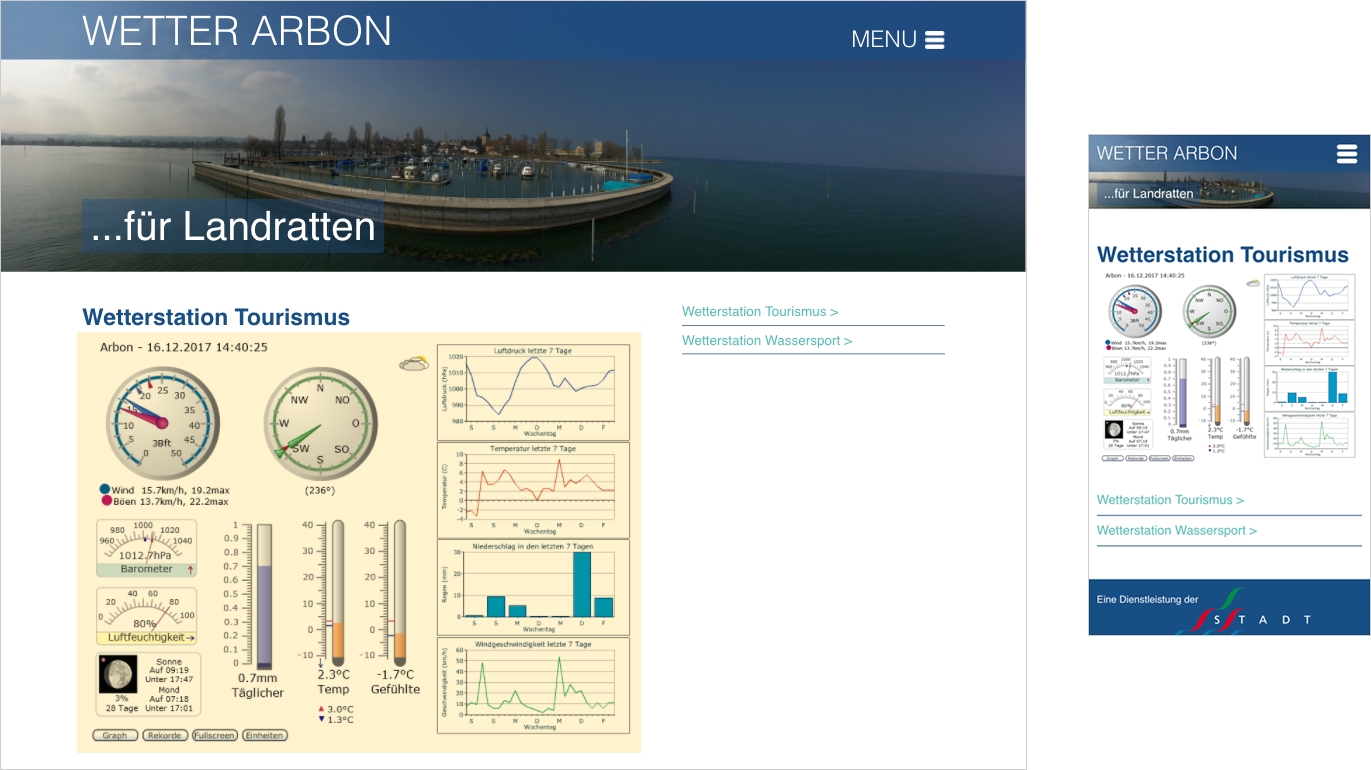
\includegraphics[width=1\linewidth]{img/responsive}
	\caption{Responsive Design: Vergleich Desktop und Mobile}
	\label{img:responsive}
\end{figure}


\noindent
%\subsubsection*{Lösungsansatz}
Mit der Adobe Flash Applikation lässt sich dieses Problem nicht lösen. Da aber, wie in Abschnitt~\ref{subsec:flash} erklärt, die Adobe Flash Applikation ohnehin abgelöst werden muss, wird bei der Ausarbeitung der neuen Anzeige darauf geachtet, dass die Wetterdaten auf allen gängigen Geräten problemlos lesbar sind. Da davon auszugehen ist, dass die Webseite häufig von Mobilgeräten aus betrachtet wird, wird das Designkonzept \textit{mobile first} angewendet. Das bedeutet, dass zuerst die Mobile-Seite designt wird und anschliessend die Desktop-Seite.


% #####################################################################################
% Darstellung der Winddaten
% ################################
\subsection{Darstellung der Winddaten}
Vielfach sind nicht nur die aktuellen Messwerte, sondern auch der Verlauf der Wetterdaten interessant. Für Segler ist beispielsweise entscheidend wie sich die Windgeschwindigkeit über die letzten paar Stunden entwickelt hat. Auf der Webseite werden deshalb neben den aktuellen Wetterdaten ausgewählte Wetterdatenverläufe dargestellt, wie in Abbildung~\ref{img:responsive} ersichtlich. Bei diesen Grafiken geht es darum die Tendenz und die Grössenordnung der Wetterdaten abschätzen zu können.
\newline

\begin{figure}[h!]
	\centering
	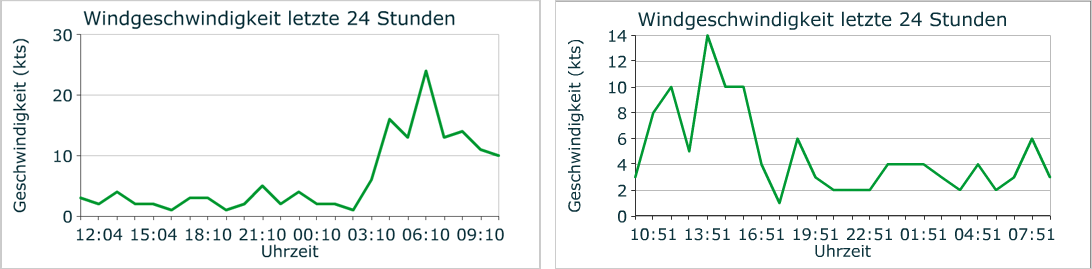
\includegraphics[width=1\linewidth]{img/wind-geschw}
	\caption{Anzeige der Windgeschwindigkeit mit variabler y-Skalierung}
	\label{img:wind-geschw}
\end{figure}

\noindent
Beim genaueren Betrachten der Verläufe von Windgeschwindigkeit und Windrichtung zeigen sich jedoch zwei Probleme.
% Windgeschwindigkeit
%\subsubsection*{Problem: Automatische y-Skalierung von Graphen}
Bei der Windstärke-Anzeige, passt sich die Skalierung der y-Achse sich je nach Windstärke automatisch an, wie Abbildung \ref{img:wind-geschw} zeigt. Das Problem ist, dass ein schnelles Ablesen der Anzeige nicht möglich ist, da die Anzeige immer zuerst in Relation zur y-Skalierung gesetzt werden muss, was mühsam ist.
\newline



\noindent
% Windrichtung
%\subsubsection*{Problem: Sprung in der Windrichtungsanzeige}
Bei der Anzeige der Windrichtung wird der zeitliche Verlauf als Linie in einem xy-Graphen dargestellt. Die y-Achse zeigt die Himmelsrichtung an, aus der der Wind kommt von 0 Grad bis 360 Grad. Das Problem bei dieser Darstellung ist, dass wenn der Wind über Norden dreht dies als Sprung in der Grafik abgebildet wird, wie in Abbildung~ \ref{img:wind-richtung} dargestellt. Durch die Interpolation der Werte entsteht so eine verwirrende und falsche Aussage.
\newline

\begin{figure}[h!]
	\centering
	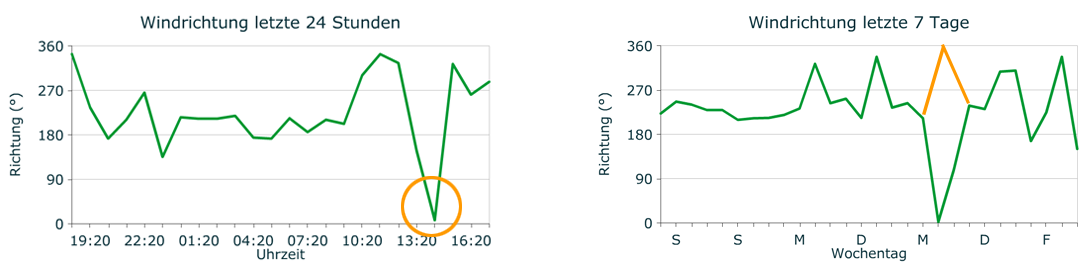
\includegraphics[width=1\linewidth]{img/wind-richtung}
	\caption{Anzeige der Windrichtung}
	\label{img:wind-richtung}
\end{figure}

\noindent
%\subsubsection*{Lösungsansatz}
Bei der Erstellung der neuen Anzeige wird darauf geachtet, dass die Graphen auf den ersten Blick eine klare Aussage zulassen indem fixe y-Skalierungen verwendet werden. Die Auswahl der Darstellungsart erfolgt zudem so, dass keine Missverständnisse bzw. Falschaussagen entstehen.



% #####################################################################################
% Sturmwarnung
% ################################
\subsection{Integration des Sturmwarndiensts}
\label{subsec:sturmwarnung}

Auf dem Bodensee gibt es einen Sturmwarndienst, der die Schiffsführer vor aufkommendem Sturm warnen soll. Der Sturmwarndienst wird vom Deutschen Wetterdienst in Zusammenarbeit mit MeteoSchweiz betrieben. Rund um den Bodensee sind dafür über 60 Sturmwarnleuchten installiert (Abbildung \ref{img:sturm2}). Diese blinken 40 mal pro Minute bei Windböen  über 25 Knoten und 90 mal pro Minute bei Windböen über 34 Knoten. Die aktuelle Warnsituation wird zudem auf der Webseite der Kantonspolizei Thurgau\footnote{ \url{http://www.kttg.ch/kapo/htm/stwarn.shtml}} als jpg-Bild publiziert, siehe Abbildung~\ref{img:sturm}, rechts. Das jpg-Bild wird direkt auf der Webseite der Wetterstation eingebunden.
\newline

\begin{figure}[h!]
	\centering
	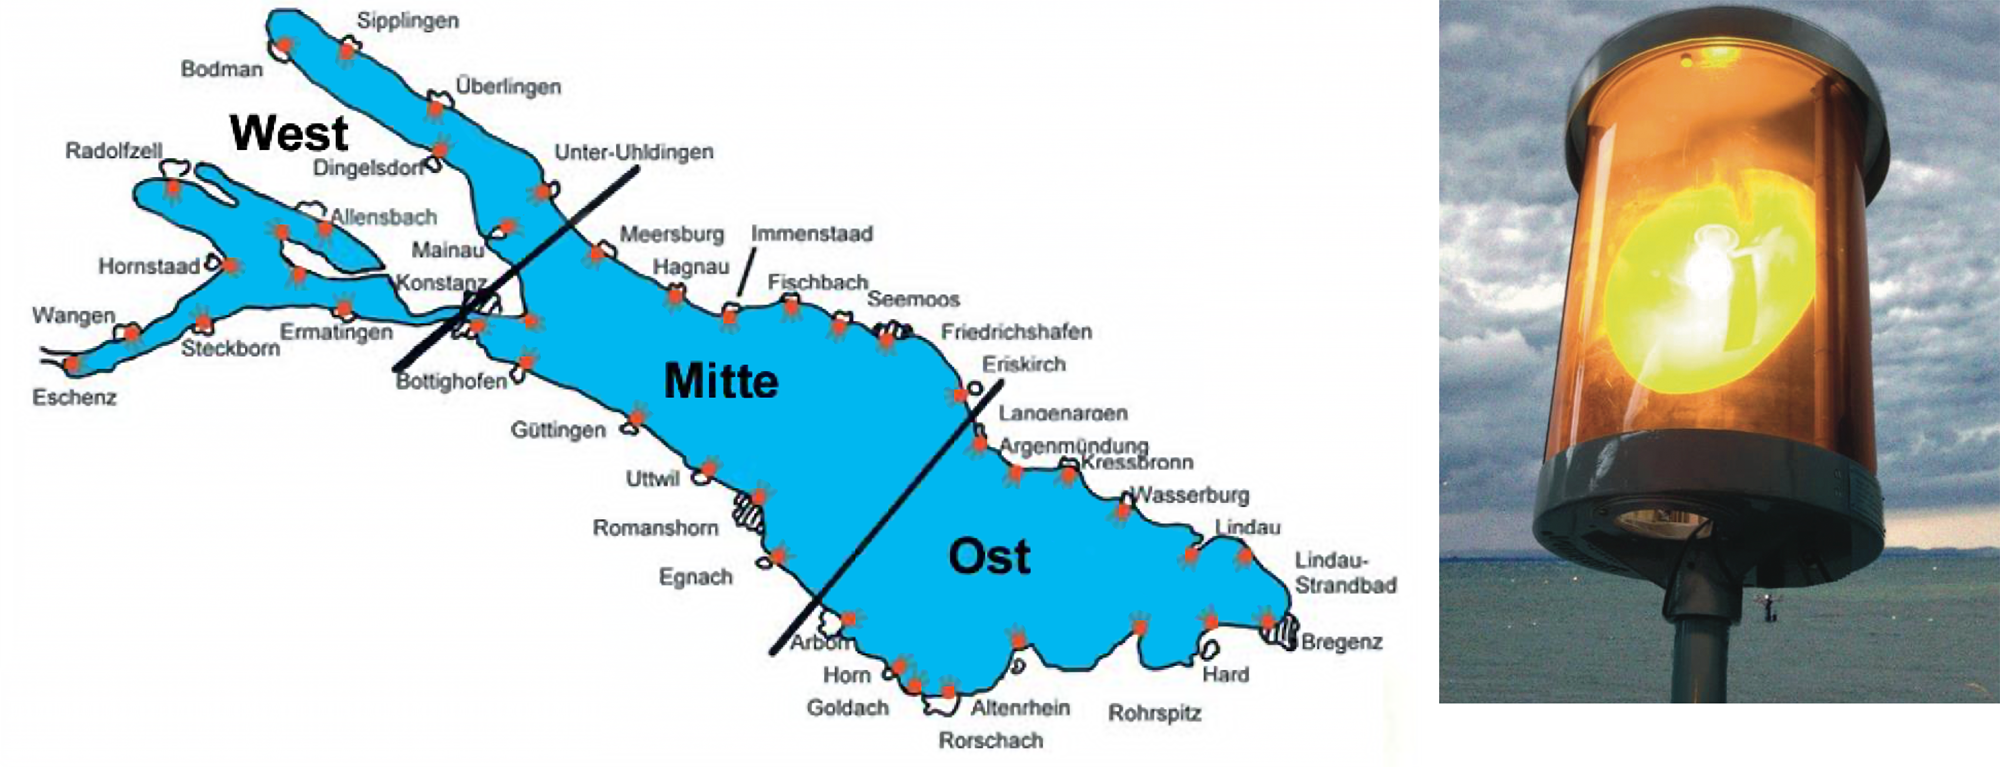
\includegraphics[width=1\linewidth]{img/sturm2}
	\caption{Sturmwarndienst Bodensee}
	\label{img:sturm2}
\end{figure}

\noindent
%\subsubsection*{Problem: HTTP}
Die Webseite der Kantonspolizei Thurgau kann nur über eine unverschlüsselte HTTP-Verbindung aufgerufen werden. Die verschlüsselte Verbindung über HTTPS wird nicht unterstützt. Google Chrome und Mozilla Firefox planen HTTP-Seiten zukünftig abzuwerten und mit einer Warnung als \flqq nicht sicher\frqq zu markieren\cite{Chromium:marking-http-as-non-secure}\cite{Mozilla:DeprecatingNon-SecureHTTP}. Für normale User ist diese Meldung nicht verständlich und erzeugt ungewolltes Misstrauen in die Webseite. 

Seit 2014 verwendet die Suchmaschine von Google zudem HTTPS als Ranking Signal. Bisher war es ein sehr schwaches Signal d.h. die Gewichtung lag bei unter einem Prozent. Google behält sich allerdings vor, die Gewichtung zu erhöhen\cite{Googleblog:https-as-ranking-signal}. Webseiten, die nicht über HTTPS verfügen werden somit in der Trefferliste weiter unten angezeigt.

\begin{figure}[h!]
	\centering
	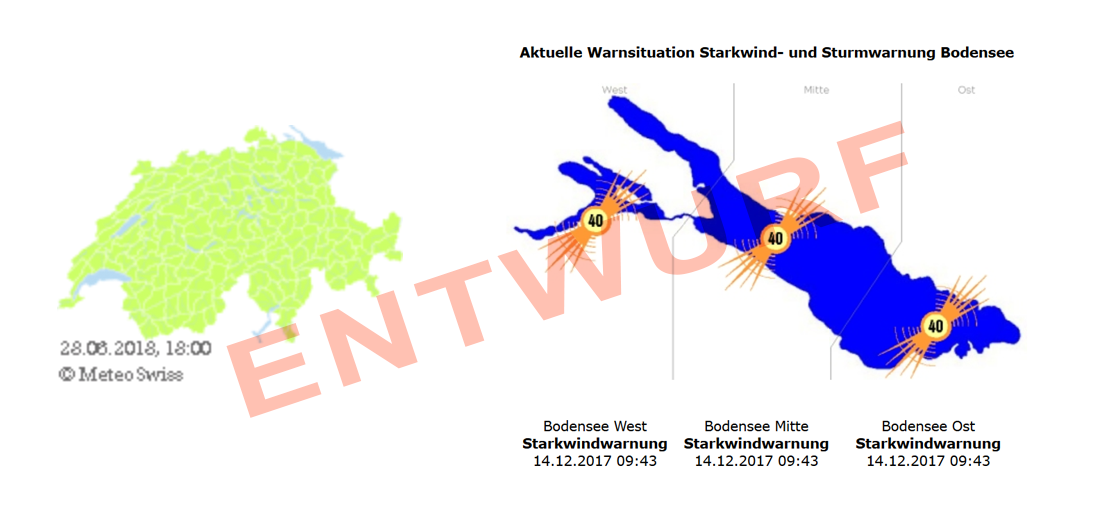
\includegraphics[width=1\linewidth]{img/sturm}
	\caption{}
	\label{img:sturm}
\end{figure}

Aus diesen beiden Gründen hat Screenbox im Herbst 2017 alle Kunden aufgefordert ihre Webseiten auf HTTPS umzustellen. Die Webseite der Wetterstation Arbon konnte problemlos umgestellt werden - mit einer Ausnahme: Da die Sturmwarnung direkt eingebettet war, konnte die Sturmwarnung-Seite der Wetterstation Arbon nicht auf HTTPS umgestellt werden. Als Sofortmassnahme wurde deshalb das eingebettete Bild entfernt und durch einen Link auf die Webseite der Kantonspolizei ersetzt, siehe Abbildung~\ref{img:sturm} links. Das dies keine langfristige Lösung sein kann, versteht sich von selbst.

%\subsubsection*{Problem: Warnzeiten}
Der Sturmwarndienst wie in Abschnitt \ref{subsec:sturmwarnung} beschrieben, ist kein 24h-Service. Der Dienst ist nur tagsüber aktiv zu den folgenden Warnzeiten\footnote{ \url{https://kapo.tg.ch/public/upload/assets/56408/A5\%20Sturmwarnung.pdf}}, was aus Sicht der Sicherheit auf dem See nicht sehr sinnvoll ist:

\begin{itemize}  
\item 1. April - 31. Oktober: 06:00 - 22:00 Uhr 
\item 1. November - 31. März: 07:00 - 20:00 Uhr
\end{itemize}

\noindent
%\subsubsection*{Lösungsansatz}
Die Information zum Sturmwarndiest des Bodensees sollen durch eine Schnittstelle abgegriffen und selbst dargestellt werden. Ob weiterhin das offizielle Signal für die Sturmleuchten, oder ein 24h-Service zum Beispiel von MeteoSchweiz verwendet werden soll, muss während der Bachelor-Arbeit mit dem Auftraggeber geklärt werden.



%
%\subsection{Probleme summiert}
%\Diskussionspunkt{
%\begin{itemize}  
%\item Flash Weiterentwicklung wird gestoppt und schon von vielen Geräten nicht mehr Unterstützt
%\item Screenshots der aktuellen Verhältnissen nicht optimal
%\item Die Skalierung der Graphen ist mehr verwirrend als hilfreich
%\item Der HTTP standard ist unsicher, wird in Zukunft eingestellt
%\end{itemize}
%}
%\sout{Das Problem der Webseite und vor allem der beiden Applikationen ist, dass viele Geräte Flash nicht mehr oder in naher Zukunft nicht mehr unterstützen. Zusätzlich ist die Lösung mit dem Screenshot der aktuellen Verhältnisse auch keine optimale Lösung. Auch sind die Schreibfehler, welche entdeckt wurden bei näherer Betrachtung auch nicht Vorteilhaft. Weiter ist die Wetterapplikation nicht nach dem Prinzip responsive Design aufgebaut, welches in der heutigen Zeit ein wichtiger Bestandteil einer Webseite ist. Zusätzlich zum Flash, von der Gebrauch gemacht wird sind die Anzeigen auf der Touristik bzw. Wassersport Seite unschön. }
%
%
%\subsection{Lösungsansatz}
%Um die Webseite auf den neusten Stand der Technik zu bringen sollten folgende Änderungen durchgeführt werden.Die Flash-Software wird ausgemustert und die Applikation wird auf HTML5 und Javascript umgestellt. Die Webseite soll zudem im responsive Design entwickelt werden, damit auch auf mobilen Geräten die aktuelle Wetterlage sichtbar ist. Die dynamischen, sowie auch die teilweise statischen Anzeigen, werden wo möglich mithilfe der Javascript Bibliothek D3.js oder Google Charts erstellt, hiermit lassen sich ansehnliche und moderne Grafiken erstellen. Die Grafiken, sollten so gestaltet sein das auch Sehbehinderte Personen erkennen wie das Wetter momentan ist. Das heisst beispielsweise, dass die Farben auch für Farbenblinde unterscheidbar sein sollten oder blinde Personen anhand eines Vorleseprogramms erkennen wie das Wetter ist. Ein weiterer Punkt ist die Auswahl der Einheiten, diese sollen nach dem ersten Besuch gespeichert bleiben beim Client mithilfe von Webstorage.

\section{Datenbank}

\Diskussionspunkt{Beginn Einlesen in DB}
Verschiedene Arten von Datenbanken:
\begin{itemize}
\item relationale DB
\item hierarchisches Datenmodell
\item Netzwerkdatenmodell
\item Objekt relationale Datenbank
\end{itemize}

Das relationale Datenmodell ist das weit verbreitetste Modell, dass hierarchische wegen der beschränkten Anwendbarkeit kaum noch vorhanden.

Vorgehen Datenbankentwicklung:

\begin{itemize}
\item Externe Phase (Ermittlung der Informationsstruktur)
\item Konzeptionelle Phase (ER-Modell)
\item Logische Phase (relationales Datenmodell)
\item Physische Phase (Erstellung des Datenmodell)
\end{itemize}

Punkte zur Überlegung neuer Datenbankstruktur:
\begin{itemize}
\item Welche Daten?
\item In welchem Intervall?
\item Welche Tabellen? (Welche Daten zusammen?, eine grosse Tabelle?)
\item Tabellennamen?
\item 
\end{itemize}

Datentypen angeschaut auf w3schoolss:
\begin{itemize}
\item Welcher Datumstyp?

\end{itemize}


Unterschied MariaDB und MySQL?\\
Wie viele Daten werden gespeichert?\\
Vor der Neukonzipierung werden täglich 1440 Datensätze gespeichert. Das bedeutet jede Minute einen Datensatz. Ein Datensatz beinhaltet 65 Einträge. Die gesamte relevante Datenbank igwetter wettertest benötigt 323.17  Mb. Die Tabelle wx data benötigt stand 1.3.18 311.94 Mb, daraus erfolgt das ein Datensatz ca 0.025 Mb benötigt \\
-Wie viele Daten können gespeichert werden?\\
Die igWetter hat bei Hostpoint einen Server mit 50 GB Speicherplatz, rechnet man die vorhergehenden Zahlen hoch mit dem zur Verfügung stehenden Speicherplatz, hat es genügend Platz für die kommenden 45 Jahren.\\

https://entwickler.de/online/datenbanken/datenbanken-grundlagen-und-entwurf-115676.html
\Diskussionspunkt{Ende Einlesen in DB}\\
\Diskussionspunkt {Beginn Einlesen DB Sicherheit}\\

Bei der Recherche nach Datenbanksicherheit taucht immer wieder das Wort Injection auf. Laut den OWASP top 10, eine Liste welche die wichtigsten Schwachstellen aufzeigt, ist die SQL-injection in 2017 auf dem Platz 1. Was ist den eigentlich SQL Injection? SQL injection ist eine Methode eine Datenbankabfrage so zu manipulieren, dass der Angreifer im schlimmsten Fall auf die gespeicherten Daten des Administators kommt. Ein anderes Beispiel wäre, dass der Angreifer an die Daten der Benutzer eines Online-Shops mit Kreditkartendaten oder ähnlichen sensitiven Daten kommt.
Weitere Fragen die auftauchen bei der Suche nach Datenbanksicherheit sind:
\begin{itemize}
\item Was für Arten von Daten beherbergt die Datenbank?
\item Hat es sensitive Daten?
\item Ist die Datenbank überhaupt ein potentielles Angriffsziel?
\item Wer sind die Benutzer der Datenbank?
\end{itemize}
Neben dem Schutz vor potentiellen Angriffen ist auch der Schutz vor Datenverlust wichtig. Dieser Schutz kann sehr einfach durch ein Backup der Datenbank umgesetzt werden. Jedoch stellen sich auch hier folgende Fragen:
\begin{itemize}
\item Welche Daten sind wichtig?
\item Wie wird das Backup umgesetzt?
\item Wie oft wird ein Backup gemacht?
\end{itemize}

\Diskussionspunkt{Ende Einlesen DB Sicherheit}\\
\Diskussionspunkt{Beginn Konzept DB Sicherheit}
In der Ausgangslage der Wetterstation und deren Datenbank wird kein Backup erstellt und ist gegen aussen nicht gesichert. Wichtig hierbei ist aber zu erwähnen, dass die Datenbank im Moment ein "Datenfriedhof" ist. Die Aufgezeichneten Daten werden nicht benutzt. Im Verlauf der Bachelorarbeit wird sich dies aber ändern, deswegen ist es für die Datenbank ist wichtig, dass Sie gegen aussen vor potentiellen Angreifern und einem Verlust der Daten beim Provider gesichert ist. \\
Das Ziel ist es die Datenbank im Vergleich zu Kosten und Aufwand sicherer zu gestalten. Es wird erwartet das ein potentieller Angreifer nicht ohne Mühe in die Datenbank eindringen kann. Des Weiteren soll bei einem allfälligen Verlust der Daten auf dem Server eine schnelle Rekonstruktion der Datenbank inklusive Daten möglich sein, damit der angebotene Service schnellst möglich wieder zugänglich ist.\\ 
Um eine Neukonzipierung zu erstellen wurde vorher eine Recherche durchgeführt. Wobei für das Konzept und die spätere Umsetzung verschiedenste Fragen aufgekommen sind. Wenn es um den erhalt der Daten, also ein Backup geht, stellen sich folgende drei Grundlegende Fragen:
 \begin{itemize}
\item Welche Daten sind wichtig?
\item Wie wird das Backup umgesetzt?
\item Wie oft wird ein Backup gemacht?
\end{itemize}

Geht es um den Schutz gegen aussen vor potentiellen Angriffen tauchen die folgenden Grundlegenden Fragen auf: 
\begin{itemize}
\item Was für Arten von Daten beherbergt die Datenbank?
\item Hat es sensitive Daten?
\item Ist die Datenbank überhaupt ein potentielles Angriffsziel?
\item Wer sind die Benutzer der Datenbank?
\end{itemize}
Sind die obenstehenden Fragen beantwortet steht auch das Konzept.\\
Um die Datenbank auch gegen einen allfälligen Datenverlust zu sichern ist ein Backup von wichtiger Bedeutung. Im Grunde sind alle Daten welche die Wetterstation ablegt von Wichtigkeit. Dabei muss aber entschieden werden, ob ein tägliches Backup Sinn machen würde. Bezüglich des Speicherplatzes und des Aufwands, da die Wetterstation von einem Verein betrieben wird, ist es wichtig den Aufwand mit dem Ertrag zu vergleichen. Ein Backup nur auf dem Server des Providers macht technisch keinen Sinn, da es auch sein kann, dass dieser mal versagt und die Daten anschliessend für immer verschwunden sind. Deswegen ist es wichtig auch ein "externes" Backup zu erstellen. Es wird empfohlen ein wöchentliches Backup zu erstellen, dies aufgrund der Datenmengen, denn wöchentlich fallen 10080 Datensätze an. Fehlt eine Woche aufgrund eines Ausfalls ist der schaden geringer als ein monatliches oder jährliches Update.\\
Das update wird mittels eines Cronejobs, welches ein Backup-Script ausführt, auf dem Server durchgeführt. Die Daten werden anschliessend in einer Cloud nach Wahl hochgeladen. Zusätzlich wird das Backup auch auf dem gemieteten Server von Hostpoint gespeichert um einen schnelleren Zugriff zu gewährleisten. Um nicht zu viele Daten "unnötig" zu speichern, wird empfohlen die Daten der vorhergehenden Woche zu überspielen. Der Nachteil dieser Lösung sind jedoch die Kosten welche bei einer \Diskussionspunkt{Cloud} anfallen. Hierbei bewegt man sich preislich bei circa 10 Franken pro Monat.

Neben der Datensicherung in Form des Backups ist auch die Sicherheit im Betrieb massgebend. Bei der Recherche nach Datenbanksicherheit taucht immer wieder das Wort Injection auf. Laut den OWASP top 10, eine Liste welche die wichtigsten Schwachstellen aufzeigt, ist die SQL-injection in 2017 auf dem Platz 1. Was ist den eigentlich SQL Injection? SQL injection ist eine Methode eine Datenbankabfrage so zu manipulieren, dass der Angreifer im schlimmsten Fall auf die gespeicherten Daten des Administators kommt. Ein anderes Beispiel wäre, dass der Angreifer an die Daten der Benutzer eines Online-Shops mit Kreditkartendaten oder ähnlichen sensitiven Daten kommt. Auf der Seite der MariaDB, welche in unserem Fall benutzt wird, werden 5 Essentielle Praktiken für die Datenbanksicherheit aufgezählt:
\begin{itemize}
\item Schütze gegen Attacken mit einem Datenbankproxy
\item Setze ein auditing und robustes logging auf
\item Praktiziere ein strenges user account management
\item Halte die Datenbanksoftware und OS up-to-date
\item Verschlüssle sensitive Daten
\end{itemize}

Die Wetterstation Arbon enthält jedoch keine sensitiven Daten. Deswegen muss die Datenbank nicht mit der höchsten Sicherheit ausgestattet sein.  Trotzdem ist Datenbank nach der Umsetzung der Bachelorarbeit eins der Herzstücke der Wetterstation. Denn diese beinhaltet die Wetterdaten jeder Minute des Tages, des Weiteren erhält sie sich auch die historischen Daten der Wetterstation. Deswegen sollte eine gewisse Grundsicherheit der Datenbank gewährleistet werden, damit die Daten nicht manipuliert bzw. die Datenbank nicht anderweitig benutzt werden kann. Die Datenbank stellt nur in dieser Hinsicht ein potentielles Ziel dar. Benutzer der Datenbank hat es im eigentlichen Sinne nur zwei. Das ist der Administrator der Seite, sowie die Webseite. Jedoch sind die Benutzer der Seite auch Benutzer der Datenbank. Doch was haben diese direkt mit der Datenbank zu tun? Auf der zukünftigen Seite der historischen Daten, sollen die Benutzer entscheiden können von wann bis wann die Daten angezeigt werden sollen. Somit müssen diese eine Abfrage tätigen.\\
Um es den Angreifern nicht zu einfach zu gestalten sollte die Abfrage gegen Injection gesichert sein. Zusätzlich ist es sinnvoll mittels logging zu erfahren welche Anfragen getätigt wurden, sowie mittels eines Cronejobs die Datenbank auf dem neusten Stand zu halten. Beim logging soll bei einer Abweichung des Verhaltens, konkret heisst dies einer veränderten Abfrage, der Verein gewarnt werden. Dies kann mittels einer E-Mail stattfinden. Da es nur einen user account für den Verein hat ist es nötig diesen mit allen Privilegien auszustatten und hieran nichts zu ändern. Des Weiteren erhält wie erwähnt die Datenbank auch keine sensitiven Daten, womit ein verschlüsseln der Daten überflüssig wird. \Diskussionspunkt{Datenbankproxy}

\Diskussionspunkt{Zusammenfassung}

Das Konzept in einer kurzen Zusammenfassung inklusive den Punkten die zur Diskussion stehen:\\
Backup:\\
Es wird ein Backup system aufgesetzt welches sicherstellt, dass die Daten einmal auf dem Server von Hostpoint sowie auf extern in einer Cloud oder sonstigem externen Speicher gespeichert werden können. Dies wird mittels einem Script von einem Cronejob wöchentlich durchgeführt. Der Diskussionspunkt ist hierbei, welche der beiden externen Varianten wird gewählt und ob die Daten in einem kürzerem oder längerem Abstand gespeichert werden.

Datenbanksicherheit:\\
Die Datenbank soll primär gegen SQL-injection gesichert werden. Des Weiteren soll geloggt werden wann welche Anfragen stattfinden und wie diese aussehen. Sollte eine Abfrage aus dem Rahmen fallen, soll der Verein mittels E-Mail oder einer sonstigen Benachrichtigung gewarnt werden. Des Weiteren soll ein Cronejob und dem dazugehörigen Skript die Software auf dem neusten Stand halten. Bei der Datenbanksicherheit steht die Benachrichtigungsart und ein eventueller Proxy wie von MariaDB empfohlen zur Diskussion. 

   



\section{Sensoren}
Die Wetterstation Arbon verfügt über fünf Sensoren bzw. Sensor-Einheiten: Webcam, Kombi-Wetter-Transmitter, Wassertemperatur-Sensor und Pegelsensor. Auf der Plattform im See draussen befindet sich lediglich ein Schaltschrank mit Datenwandlern und keine Auswerteeinheit. Sämtliche Daten werden per TCP/IP an den Server geschickt. Abbildung \ref{img:schaltschrank} zeigt den schematischen Aufbau der Komponenten im Schaltschrank und die angeschlossenen Sensoren. Die Stromversorgung ist der Übersicht halber nicht dargestellt.

\begin{figure}[h]
	\centering
	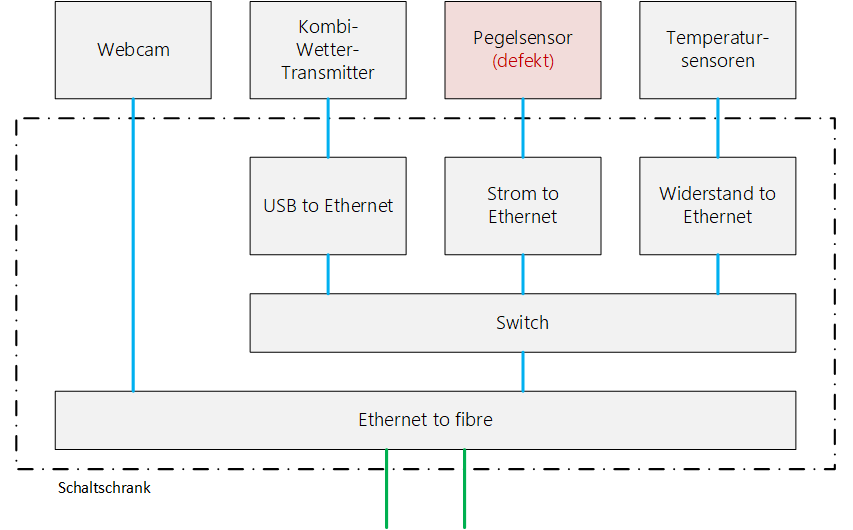
\includegraphics[width=1\linewidth]{img/schaltschrank}
	\caption{Hardware-Aufbau der Wetterstation Arbon}
	\label{img:schaltschrank}
\end{figure}



\subsection{Pegelmesser}
Der bisherige Pegel-Sensor nutzte das Prinzip der hydrostatischen Druckmessung. Der Sensor ist nun aber defekt und muss ersetzt werden. Neben der hydrostatischen Druckmessung kommen weitere potentielle Messprinzipien in Fragen. Sie alle erfüllen die Grundanforderung bezüglich Messdistanz und Robustheit. Während der Bachelor-Arbeit wird der passende Pegelsensor getestet und ausgewählt. Möglich ist:

\begin{itemize}  
\item Hydrostatische Druckmessung
\item Ultraschall-Distanzmessung
\item Radar-Distanzmessung
\item Time-of-flight-Distanzmessung
\end{itemize}

\subsection{Wassertemperatursensoren}
Die Wassertemperatur wird definitionsgemäss einen Meter unterhalb der Wasseroberfläche gemessen. Die Wetterstation Arbon verwendet eine Widerstandskaskade aus PT100-Widerständen. Diese sind in einem Kunststoffrohr im Abstand von 20cm angeordnet. Abhängig vom gemessenen Pegel kann so der richtige Temperatursensor für die Wassertemperatur ausgewählt werden. Von den zehn verbauten Sensoren ist einer defekt. Da die Reparatur allerdings sehr aufwändig ist, und der Wert durch die beiden Nachbarwiderstände interpoliert werden kann, wird der Widerstand nicht ersetzt. Für uns besteht diesbezüglich kein Handlungsbedarf.













 
%%%%%%%%%%%%%%%%%%%%%%%%%%%%%%%%%%%
%%  Webcam
%%%%%%%%%%%%%%%%%%%%%%%%%%%%%%%%%%%
\section{Webcam-Steuerung}
Zur Wetterstation Arbon gehört eine schwenk- und zoombare Webcam. Diese ist über ein Applikations-Plugin in die Webseite integriert. In der Titelleiste sind zusätzlich die wichtigsten Wetterdaten aufgeführt, wobei die Einheit der Windgeschwindigkeit jeweils alle dreissig Sekunden zwischen km/h und Knoten wechselt. Die Webseite der Webcam ist in Abbildung \ref{img:warteschlange} links dargestellt.

\begin{figure}[h]
	\centering
	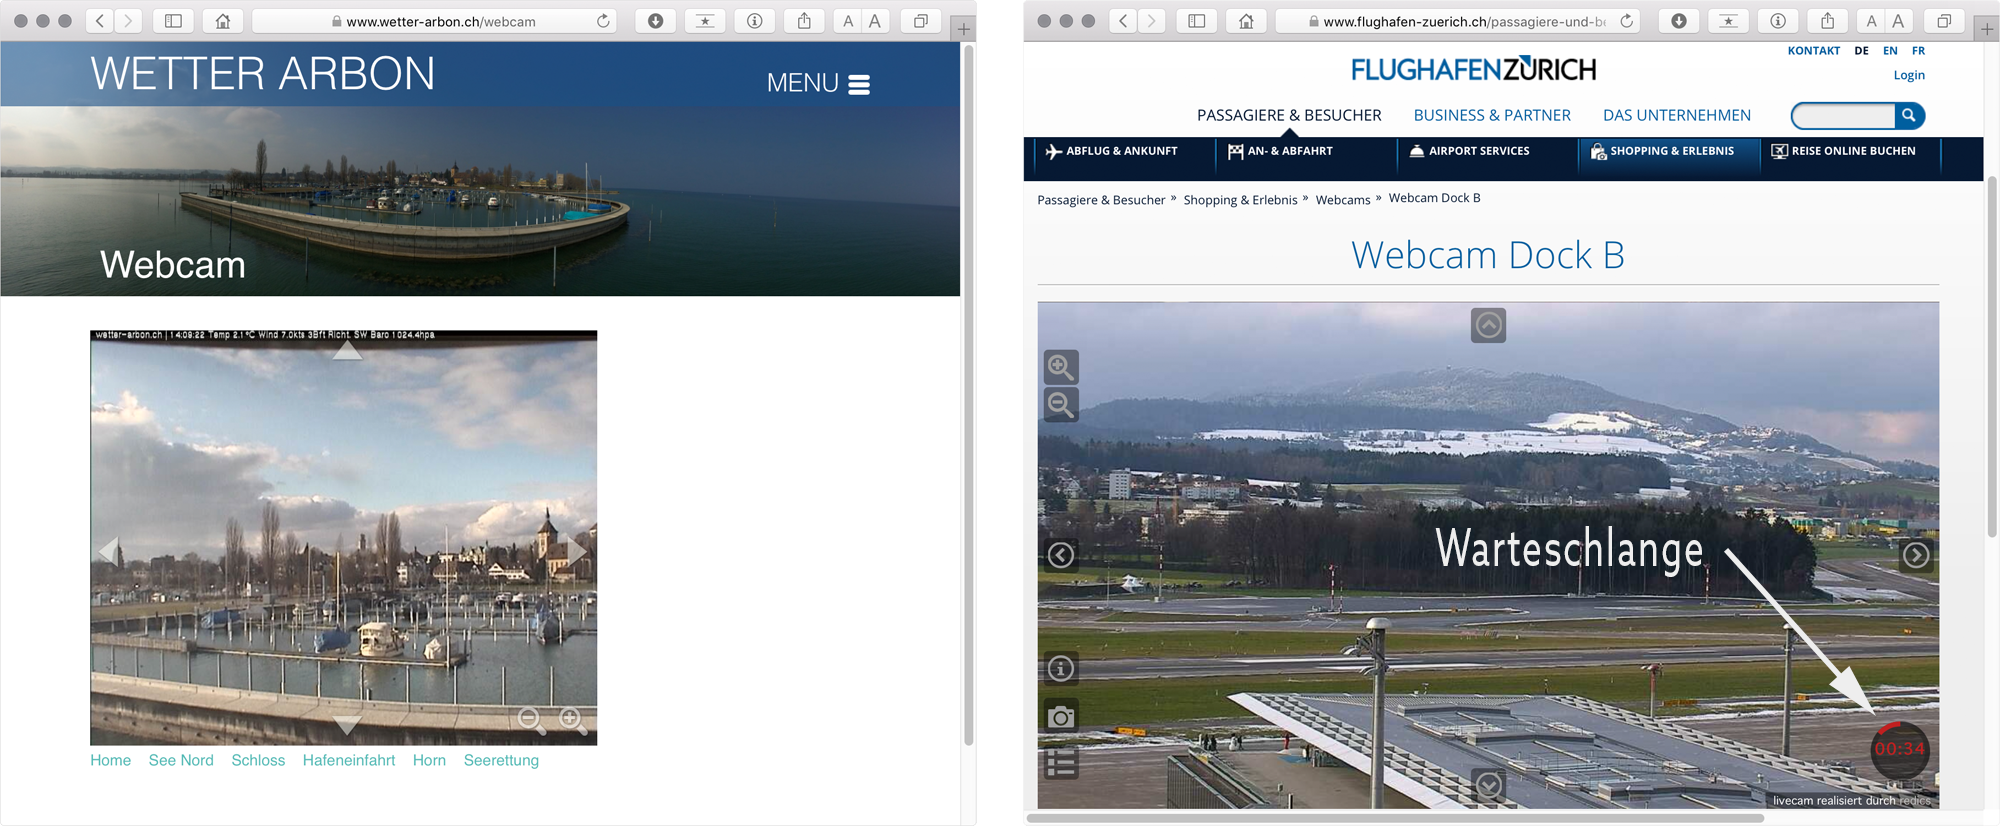
\includegraphics[width=1\linewidth]{img/warteschlange}
	\caption{Webcam Arbon und Beispiel einer Warteschlange}
	\label{img:warteschlange}
\end{figure}


% Warteschlange
\subsection{Warteschlange für Webcam-Steuerung}
Der Benutzer hat die Möglichkeit die Webcam nach oben/unten und nach links/rechts zu bewegen. Sechs voreingestellte Positionen stehen als Shortlinks zur Verfügung. Diese Positionen sind in der betriebseigenen Software der Webcam konfigurierbar.
\newline

%Die freie Positionierung erfolgt über Pfeile, sowie die Plus und Minus am Bildrand, je nachdem welcher Button geklickt wird, sendet die Webseite das Kommando mittels HTTP an die Webcam. Die Zusammenstellung des URLs geschieht über ein Javascript, wie man dem Code in Listing \ref{lst:cam} entnehmen kann.

%\begin{lstlisting}[caption={Positionsänderung der Webcam},label={lst:cam},language=html]
% <div class="container webcam" id="webcam_585">
%	<img class="pageImage" src="https://webcam.wetter-arbon.ch/mjpg/video.mjpg"/>
%</div>
%<script type="text/javascript">
%	function changeWebCam(command) {
%		var urlAddition;
%		switch (command) {
%			case 'up':
%			case 'down':
%			case 'left':
%			case 'right':
%			case 'home':
%				urlAddition = 'move=' + command;
%				break;
%				
%			case 'zoomIn':
%				urlAddition = 'rzoom=2500';
%				break;
%				
%			case 'zoomOut':
%				urlAddition = 'rzoom=-2500';
%				break;
%				
%			case 'Hafeneinfahrt':
%				urlAddition = 'gotoserverpresetname=' + command;
%				break;		
%		}
%		console.log('changeWebCam');
%		$.get('https://webcam.wetter-arbon.ch/axis-cgi/com/ptz.cgi?camera=1&' + urlAddition);
%	}
%\end{lstlisting}


\noindent
%\subsection*{Problem}
Die Möglichkeit der Webcam-Steuerung übers Web ist zwar sehr attraktiv, hat aber auch seine Nachteile. Zum Beispiel wenn mehrere Personen gleichzeitig auf die Webcam zugreifen. Zur Zeit ist es so dass, die HTTP-Request der Reihe nach abgearbeitet werden. Es ist also möglich, dass sich die Benutzer gegenseitig in der Bedienung stören, was unter Umständen recht mühsam ist. 
\newline

\noindent
%\subsection*{Lösungsansatz}
Das Prinzip der Warteschlange kann hier Abhilfe schaffen. Jeder Benutzer erhält eine bestimmte Zeit den alleinigen Zugriff auf die Steuerung der Webcam. So eine Lösung setzt zum Beispiel der Flughaben Zürich\footnote{ \url{https://www.flughafen-zuerich.ch/passagiere-und-besucher/shopping-und-erlebnis/webcams/webcam-dock-b}} ein, wie in Abbildung \ref{img:warteschlange} rechts dargestellt.



% Zoom
\subsection{Positionsabhängige Zoombeschränkung}
In der betriebseigenen Software der Webcam lassen sich viele Parameter konfigurieren, unter anderem der Zoomfaktor. 
\newline

\noindent
%\subsection*{Problem}
Das Problem ist, dass der Zoomfaktor nur allgemein eingestellt werden kann, das heisst die Beschränkung gilt immer, egal ob die Kamera auf eine Wohnung zeigt oder auf den See raus. Aus Persönlichkeitsschutz-Gründen musste deshalb der Zoomfaktor auf die 4-fache Vergrösserung limitiert werden, möglich wäre aber eine 216-fache Vergrösserung. Daraus wird deutlich, dass die Webcam eigentlich ein viel grösseres Potential hätte.
\newline

\noindent
%\subsection*{Lösungsansatz}
Die Idee ist nun die Limitierung des Zooms so zu programmieren, dass diese möglichst dynamisch ist. Das heisst, dass je nach Position die Zoom-Limitierung ändert. Der Zoom soll, vor allem auf den See hinaus, in vollem Umfang genutzt werden können. Zudem darf die Funktion nicht umgangen werden können.



\section{Erweiterungen}
In diesem Kapitel geht es nicht um die Verbesserung von bestehenden Problemen, sondern um die Erweiterung des Funktionsumfangs der Wetterstation Arbon. Es ist eine Auflistung möglicher Erweiterungen.

% Benachrichtigungen
\subsection{Individueller Benachrichtigungs-Service}
Mit einem Benachrichtigungs-Service soll dem Benutzer die Möglichkeit gegeben werden, dass er zeitnah über Wetteränderungen informiert wird und somit keine Warnung oder sein perfektes Segelwetter verpasst. Dafür wurden drei verschiedene Möglichkeiten ausgewählt und mit der Nutzwertanalyse ausgewertet. Ziel bei allen Möglichkeiten ist es, dass der Benutzer die Möglichkeit hat Alarmkriterien selbst zu bestimmen. Werden die gewählten Alarmkriterien erreicht bzw. wird eine Sturmwarnung herausgegeben, wird der Benutzer benachrichtigt. Für die Evaluierung der Notifications wurde eine Nutzwertanalyse (Tabelle \ref{table:nutzwertanalyse}) erstellt. Dies ist eine gute Möglichkeit, um verschiedene Lösungsansätze zu bewerten. Der Nachteil hierbei ist jedoch, dass die Bewertung sehr subjektiv ist. Aus der Nutzwertanalyse geht hervor, dass die Benachrichtigung per E-Mail und Facebook Messenger die Lösungsansätze mit der höchsten Punktzahl sind . Der grösste Vorteil der beiden möglichen Lösungen sind, dass sie kostenlos sind. Der Nachteil an Facebook Messenger ist, dass nicht davon ausgegangen werden kann, dass jeder Benutzer ein Facebookprofil hat. 

\begin{table}
\begin{center}
\begin{tabular}{ |p{3.5cm}||p{1.1cm}|p{2cm}|p{1.7cm}|p{2.3cm}|p{1.4cm}|}
 \hline
 \multicolumn{6}{|c|}{Nutzwertanalyse} \\
 \hline
	Möglichkeiten & Kosten & Einfachheit & Aufwand & Anpassbarkeit & Support\\
 \hline
	SMS & 1 & 4 & 3 & 3 & 5\\
	E-Mail & 5 & 4 & 5 & 5 & 1\\
	FacebookMessenger & 5 & 4 & 3 & 4 & 1\\
 
\hline
\end{tabular}
\end{center}
\caption{Nutzwertanalyse verschiedner Notifikations-Möglichkeiten}
\label{table:nutzwertanalyse}
\end{table}


% Windprognose-Genauigkeit
\subsection{Überprüfung der Windprognose-Genauigkeit }
Es gibt diverse Anbieter von Windprognosen für den Bodensee wie zum Beispiel Windfinder\footnote{ \url{https://www.windfinder.com/forecast/arbon}} und SRF Meteo\footnote{ \url{https://www.srf.ch/meteo/surf-und-segelwetter/detail/06621}}. Vorhersagen sind Extrapolationen von Wettermodell-Berechnungen und mit gewissen Unsicherheiten behaftet. Interessant ist nun zu wissen wie gut die Windvorhersagen mit den Wind-Messwerten der Wetterstation Arbon übereinstimmen. Während der Bachleor-Arbeit soll eine Vergleichsgrafik erstellt werden, welche die Vorhersage den Messwerten gegenüber stellt.


% Wellenhöhe
\subsection{Berechnung und Darstellung der Wellenhöhe}
Sobald ein funktionstüchtiger Pegelsensor installiert ist, können die Pegeldaten auch für andere Zwecke verwendet werden, zum Beispiel zur Berechnung der Wellenhöhe. Dies ist insbesondere für Motorboot-Fahrer interessant.


% Schichtung Wassertemperatur
\subsection{Verlauf der Wassertemperatur in Abhängigkeit der Tiefe}
Die Wetterstation Arbon verfügt über mehrere Temperatursensoren, die im Abstand von 50 Zentimeter die Wassertemperatur messen. Die Idee ist, die Temperaturschichtung des Wassers bestimmen zu können.


% API
\subsection{Schnittstelle zu den aktuellen Messwerten (API)}
Die Wetterstation Arbon misst die Lufttemperatur und die Wassertemperatur des Bodensees. Die Badi Arbon, welche ca. einen Kilometer von der Wetterstation entfernt ist, zeigt auf ihrer Infotafel und auf ihrer Webseite\footnote{ \url{https://www.schwimmbad-arbon.ch}} ebenfalls die Luft- und Wassertemperatur an, bezieht diese aber von \textit{openWeatherMap}, welche die Temperaturen von Stationen aus Zürich und Friedrichshafen interpoliert. 
\newline

\noindent
%\subsection*{Problem: Unterschiedliche Werte für Luft- und Wassertemperatur}
Dass die gemessenen Werte der Wetterstation nicht mit den interpolierten Werten von Zürich und Friedrichshafen übereinstimmt ist nicht verwunderlich. Für der Bevölkerung ist die Differenz jedoch unverständlich. Die Stadt Arbon möchte deshalb, dass die Badi die Messwerte der Wetterstation nutzen kann.
\newline

\noindent
%\subsection*{Lösungsansatz}
Die aktuellen Werte der Wetterstation sollen über ein REST Web-API von Dritten, wie zum Beispiel der Badi Arbon, abgerufen werden können. Das heute am meisten verwendete Format dafür ist JSON.


\section{Anforderungen}
Die im folgenden aufgelisteten Anforderungen sind in fünf Blöcke unterteilt: User Interface, Datenbank, Sensoren, Webcam und nicht-funktionale Anforderungen.
Jede Anforderung besitzt eine eindeutige Identifizierungsnummer, Titel, Beschreibung der Anforderung, Wichtigkeit und einen Beschrieb wie der Nachweis erfolgen soll.
Die Wichtigkeit ist MUSS, SOLL oder KANN. MUSS-Anforderungen sind absolut zwingend für die Umsetzung der Arbeit. SOLL-Anforderungen bringen einen erheblichen Mehrwert und KANN-Anforderungen sind eher unwichtig und können gegebenenfalls auch weggelassen werden.

% ###############################################
%. Anforderungen zum User Interface
% ###############################################
\subsection{User Interface (UI)}
% 
\begin{usecase}
  \addheading{UI 010}{Flash-less Webseite (FA)} 
  \addrow{Anforderung}{Sämtliche Webseiten der Wetterstation Arbon funktionieren ohne direkte bzw. indirekte Verwendung von Adobe Flash.}
  \addrow{Wichtigkeit}{MUSS}
  \addrow{Test}{Sämtliche Webseiten der Wetterstation Arbon können von folgenden Browsern angezeigt werden, ohne dass Adobe Flash aktiviert bzw. installiert ist: Safari (Mobile \& Desktop), Google Chrome (Mobile \& Desktop), Firefox, Edge und Internet Explorer. }
\end{usecase}
% 
\begin{usecase}
  \addheading{UI 020}{Einheiten} 
  \addrow{Anforderung}{Für die Anzeige der Messwerte werden folgende Einheiten verwendet: Temperatur in C, Luftdruck in hPa, Windrichtung mindestens in Grad, Niederschlagsmenge in mm, Relative Luftfeuchtigkeit in \% }
  \addrow{Wichtigkeit}{MUSS}
  \addrow{Test}{Die Messwerte werden in C, hPa, Grad, mm und \% angezeigt. }
\end{usecase}
% 
\begin{usecase}
  \addheading{UI 030}{Wetterdaten für Wassersportler} 
  \addrow{Anforderung}{Die Anzeige der Wettertransmitterdaten erfolgt in nautischen Einheiten d.h. die Windgeschwindigkeit wird in Knoten angegeben und parallel dazu in Beaufort. Graphen zeigen den Verlauf von Luftdruck, Windgeschwindigkeit und Windrichtung der letzten 24h auf.}
  \addrow{Wichtigkeit}{MUSS}
  \addrow{Test}{Die aktuelle Windgeschwindigkeit wird auf der Wassersport-Seite in Knoten und Beaufort angegeben. Die x-Achse der Graphen zeigt die letzten 24h. }
\end{usecase}
% 
\begin{usecase}
  \addheading{UI 040}{Wetterdaten für Tourismus} 
  \addrow{Anforderung}{Die Anzeige der Wettertransmitterdaten erfolgt in allgemein verständlichen Einheiten d.h. die Windgeschwindigkeit wird in km/h angeben. Graphen zeigen den Verlauf von Temperatur, Niederschlag und Windchill der letzten sieben Tage auf. }
  \addrow{Wichtigkeit}{MUSS}
  \addrow{Test}{Die Windgeschwindigkeit wird in km/h angezeigt. Die x-Achse der Graphen zeigt die letzten sieben Tage. }
\end{usecase}
% 
\begin{usecase}
  \addheading{UI 050}{Responsive Design} 
  \addrow{Anforderung}{Die Werte der Wetterstation sind unabhängig von der Bildschirmgrösse übersichtlich und lesbar dargestellt. Horizontales Scrollen ist nicht erforderlich.}
  \addrow{Wichtigkeit}{SOLL}
  \addrow{Test}{Die Webseite der Wetterdaten wird mit einem iPhone 5, iPad und Desktop so dargestellt, dass kein horizontaler Scrollbalken auftritt.}
\end{usecase}
% 
\begin{usecase}
  \addheading{UI 060}{Samplerate} 
  \addrow{Anforderung}{Die Sample-Rate der Graphen ist kleiner gleich zehn Minuten auf der Wassersport-Seite und kleiner gleich eine Stunde auf der Tourismus-Seite.}
  \addrow{Wichtigkeit}{SOLL}
  \addrow{Test}{Pro Graph sind für die Wassersport-Seite mindestens 24*6=144 Punkte eingezeichnet, für die Tourismus-Seite mindestens 7*24=168 Werte.}
\end{usecase}
% 
\begin{usecase}
  \addheading{UI 070}{Fixe Y-Achse} 
  \addrow{Anforderung}{Für die Graphen auf der Tourismus und Wassersport-Seite wird eine fixe Y-Achs-Skalierung verwendet.}
  \addrow{Wichtigkeit}{SOLL}
  \addrow{Test}{Unabhängig von den Messwerten ist die Skalierung der y-Achse sämtlicher Graphen auf der Tourismus- und Wassersport-Seite konstant.}
\end{usecase}
% 
\begin{usecase}
  \addheading{UI 080}{Anzeige Windrichtung} 
  \addrow{Anforderung}{Die Anzeige der Windrichtung kann sich kontinuierlich ändern, ohne dass in der Momentananzeige bzw. im Graphen ein Sprung entsteht.}
  \addrow{Wichtigkeit}{SOLL}
  \addrow{Test}{Wenn sich der Wind einem um 360 Grad dreht ist auf der Anzeige und im Graphen keine Sprung erkennbar.}
\end{usecase}
% 
\begin{usecase}
  \addheading{UI 090}{Barrierefreiheit} 
  \addrow{Anforderung}{Die Anzeige der Wetterstation soll sowohl mit rot/grün Sehschwäche, als auch für sehbehinderte Menschen verständlich sein.}
  \addrow{Wichtigkeit}{SOLL}
  \addrow{Test}{Die Seiten werden mit einem Online-Color-Checker und einem Screen-Reader auf deren Verständlichkeit überprüft}
\end{usecase}
% 
\begin{usecase}
  \addheading{UI 100}{Notification} 
  \addrow{Anforderung}{Der User kann sich selbst eine Notifikation einrichten. Er erhält eine Nachricht sobald der von ihm definierte Wert der Wetterstation unter- bzw. überschritten wird}
  \addrow{Wichtigkeit}{KANN}
  \addrow{Test}{Der User richtet sich eine Notification ein für Wassertemperatur grösser als 20 Grad und Windgeschwindigkeit grösser 10 Knoten und erhält für jede Anweisung eine separate Nachricht, sobald diese erfüllt ist.}
\end{usecase}
% 
\begin{usecase}
  \addheading{UI 110}{Favicon} 
  \addrow{Anforderung}{Wenn die Webseite auf dem Homescreen eines Mobilgerätes abgespeichert wird, ist das Favicon der Wetterstation Arbon abgebildet.}
  \addrow{Wichtigkeit}{KANN}
  \addrow{Test}{Der User speichert die Webseite auf einem iPhone und sieht das Wetterstation Arbon Favicon}
\end{usecase}


% ###############################################
%. Anforderungen zur Datenbank
% ###############################################
\subsection{Datenbank (DB)}
\begin{usecase}
  \addheading{DB 010}{Abfrage-Seite} 
  \addrow{Anforderung}{Auf der Webseite der Wetterstation Arbon gibt es eine eigene Seite, auf der vom User Datenbank-Abfragen ausgeführt werden können. Das Resultat wird jeweils graphisch dargestellt. Die Abfragen können auf sämtliche Messwerte der Wetterstation und über den Zeitraum seit Datenerfassung durchgeführt werden. Liegen für einen bestimmten Zeitraum keine Messwerte vor, werden keine Werte angezeigt, und es findet auch keine Interpolation statt.}
  \addrow{Wichtigkeit}{MUSS}
  \addrow{Test}{Der User macht zwei Abfragen: In der ersten Abfrage soll die Windgeschwindigkeit in km/h seit Messbeginn aufgezeichnet werden. In der zweiten Abfrage soll der Pegel im ersten Betriebsjahr aufgezeichnet werden. Die Werte werden korrekt in der Grafik abgebildet inkl. Messlücke.}
\end{usecase}
%
\begin{usecase}
  \addheading{DB 020}{Schutz vor Missbrauch} 
  \addrow{Anforderung}{Die Schnittstelle zur Datenbank d.h. die Datenbank-Abfrage ist gegen schädliche Zugriffe geschützt.}
  \addrow{Wichtigkeit}{MUSS}
  \addrow{Test}{Die Abfrage des Pegels seit Inbetriebnahme der Wetterstation wird als File exportier und kann anschliessend in Excel geöffnet werden.}
\end{usecase}
%
\begin{usecase}
  \addheading{DB 030}{Fehleingaben} 
  \addrow{Anforderung}{Die Abfrage-Seite ist so ausgeführt, dass sie Fehleingaben verunmöglicht.}
  \addrow{Wichtigkeit}{MUSS}
  \addrow{Test}{Der User versucht eine unplausible Abfrage zu senden.}
\end{usecase}
%
\begin{usecase}
  \addheading{DB 040}{Datenmanagement} 
  \addrow{Anforderung}{Die Daten in der Datenbank werden periodisch ausgedünnt d.h. zusammengefasst.}
  \addrow{Wichtigkeit}{SOLL}
  \addrow{Test}{Messwerte, die älter als eine Woche sind, werden zusammengefasst zu maximal einem Wert pro Stunde.}
\end{usecase}
%
\begin{usecase}
  \addheading{DB 050}{Daten-Export} 
  \addrow{Anforderung}{Die Resultate der getätigten Abfragen können als Datei exportiert werden.}
  \addrow{Wichtigkeit}{KANN}
  \addrow{Test}{}
\end{usecase}


% ###############################################
%. Anforderungen zu den Sensoren
% ###############################################
\subsection{Sensoren (TD)}
\begin{usecase}
  \addheading{TD 010}{Pegel-Messer} 
  \addrow{Anforderung}{Die Wetterstation Arbon erhält einen geeigneten Pegel-Sensor, welcher mit den bereits verbauten Komponenten betrieben werden kann. Die Kosten für Anschaffung und Betrieb des neuen Sensors lieben innerhalb des Budgets der Wetterstation Arbon.}
  \addrow{Wichtigkeit}{MUSS}
  \addrow{Test}{Der Pegel Arbon wird auf der Station gemessen und ist auf der Webseite ersichtlich.}
\end{usecase}
%
\begin{usecase}
  \addheading{TD 020}{Schnittstelle zur Wassertemperatur} 
  \addrow{Anforderung}{Die Wetterstation Arbon verfügt über eine öffentlich nutzbar Schnittstelle (API) für die Wassertemperatur, sodass z.B. das Seebad diese übernehmen kann.}
  \addrow{Wichtigkeit}{MUSS}
  \addrow{Test}{Die Wassertemperatur kann über ein API abgerufen werden.}
\end{usecase}
%
\begin{usecase}
  \addheading{TD 030}{Sturmwarnung} 
  \addrow{Anforderung}{Auf der Webseite wird die aktuelle Sturmwarn-Situtation dargestellt. Falls es sich um eine engebettete Seite handelt, muss diese https-fähig sein.}
  \addrow{Wichtigkeit}{SOLL}
  \addrow{Test}{Die aktuelle Sturmwarn-Situation ist für den User auf der Webseite der Wetterstation Arbon einsehbar, ohne Verlinkung auf fremde Seiten.}
\end{usecase}
%
\begin{usecase}
  \addheading{TD 040}{Vergleich Windvorhersage und Windmessresultate} 
  \addrow{Anforderung}{Auf der Webseite ist grafisch ersichtlich wie die Windgeschwindigkeits-Vorhersage und die gemessene Windgeschwindigkeit zueinander stehen.}
  \addrow{Wichtigkeit}{SOLL}
  \addrow{Test}{Die vorhergesagten und die gemessenen Windgeschwindigkeiten der letzten sieben Tage sind grafisch dargestellt.}
\end{usecase}
%
\begin{usecase}
  \addheading{TD 050}{Wellenhöhen} 
  \addrow{Anforderung}{Aus den Messwerten des Pegelsensors wird die durchschnittliche Wellenhöhe berechnet und angezeigt. Die Wellenhöhe wird in der Datenbank gespeichert.}
  \addrow{Wichtigkeit}{SOLL}
  \addrow{Test}{Der User sieht auf der Webseite die aktuelle Wellenhöhe. Der User führt eine Datenbankabfrage aus und sieht den Verlauf der Wellenhöhe über die letzten drei Monate.}
\end{usecase}
%
\begin{usecase}
  \addheading{TD 060}{Strahlungssensor} 
  \addrow{Anforderung}{Die Wetterstation Arbon erhält einen geeigneten Sonnenstrahlungs-Sensor. Die Kosten für Anschaffung und Betrieb des neuen Sensors lieben innerhalb des Budgets der Wetterstation Arbon.}
  \addrow{Wichtigkeit}{KANN}
  \addrow{Test}{Die Sonnenstrahlung wird auf der Station gemessen und ist auf der Webseite ersichtlich.}
\end{usecase}


% ###############################################
%. Anforderungen zur Webcam
% ###############################################
\subsection{Webcam (CA)}
\begin{usecase}
  \addheading{CA 010}{Warteschlange} 
  \addrow{Anforderung}{Die Webcam verfügt über eine Warteschlage, sodass wenn mehrere User auf der Seite sind, jeder die Steuerung der Webcam für eine gewisse Zeit für sich alleine hat.}
  \addrow{Wichtigkeit}{SOLL}
  \addrow{Test}{Zwei User greifen zur gleichen Zeit auf die Webcam zu. Der zweite erhält die Steuerung, sobald die Zeit des ersten Users abgelaufen ist.}
\end{usecase}
%
\begin{usecase}
  \addheading{CA 020}{Sekotrweise Zoombeschränkung} 
  \addrow{Anforderung}{Die Zoomstufe ist abhängig von der Ausrichtung der Webcam. Richtung Land ist der Zoom beschränkt, Richtung See offen.}
  \addrow{Wichtigkeit}{KANN}
  \addrow{Test}{Der User zoomt einmal maximal Richtung Land und einmal maximal Richtung See. Die Zoomstufe Richtung Land ist kleiner, als Richtung See.}
\end{usecase}


% ###############################################
%. Nicht Funktionale Anforderungen
% ###############################################
\subsection{Nicht Funktionale Anforderungen (NF)}
\begin{usecase}
  \addheading{NF 010}{Reaktionsgeschwindigkeit} 
  \addrow{Anforderung}{Bei ausreichendem Netz werden die Messdaten innerhalb von drei Sekunden angezeigt. Datenbank-Abfragen werden innerhalb von fünf Sekunden angezeigt.}
  \addrow{Wichtigkeit}{SOLL}
  \addrow{Test}{Der User ruft die Seite auf und sieht die Messresultate innerhalb von drei Sekunden. Der User wählt die Wassertemperatur der letzten zwölf Monate und erhält fünf Sekunden nach absenden der Abfrage das Resultat.}
\end{usecase}




















   
\section{Projektmanagement}
Wir wollen das Projektmanagement schlank halten um möglichst viel Zeit in die Entwicklung der Artefakte stecken zu können.
Dieser Grundgedanke hat uns bei der im Folgenden beschrieben Auswahl der Modelle und Prozesse geleitet.

% ################################
% Vorgehensmodell
% ################################
\subsection{Vorgehensmodell}

Die Anforderungen an das Vorgehensmodell haben wir folgendermassen definiert:
\begin{itemize}  
\item wenig administrativer Aufwand, schlank
\item passend zur Projektgrösse
\item kompatibel mit den NTB-Vorgaben (Aufteilung Fachmodul, Bachelor-Arbeit)
\end{itemize}

Schnell merkten wir, dass die heutzutage beliebten agilen Vorgehensmodelle wie XP oder Scrum für uns ein Overkill darstellen und aus mehrerer Hinsicht nicht geeignet sind. Bei der Bachelor-Arbeit sind die Anforderungen im Fachmodul-Bericht definiert und ändern sich während der Bachelor-Arbeit nicht mehr. Die zu bearbeitenden Themen-Blöcke weisen untereinander nur sehr wenige Schnittstellen auf und können dadurch als eigenständige Teilprojekte das Modell durchlaufen. Unser Team besteht zudem nur aus zwei Personen, was den Koordinationsaufwand auf ein minimum reduziert.

\begin{figure}[htbp]
	\centering
	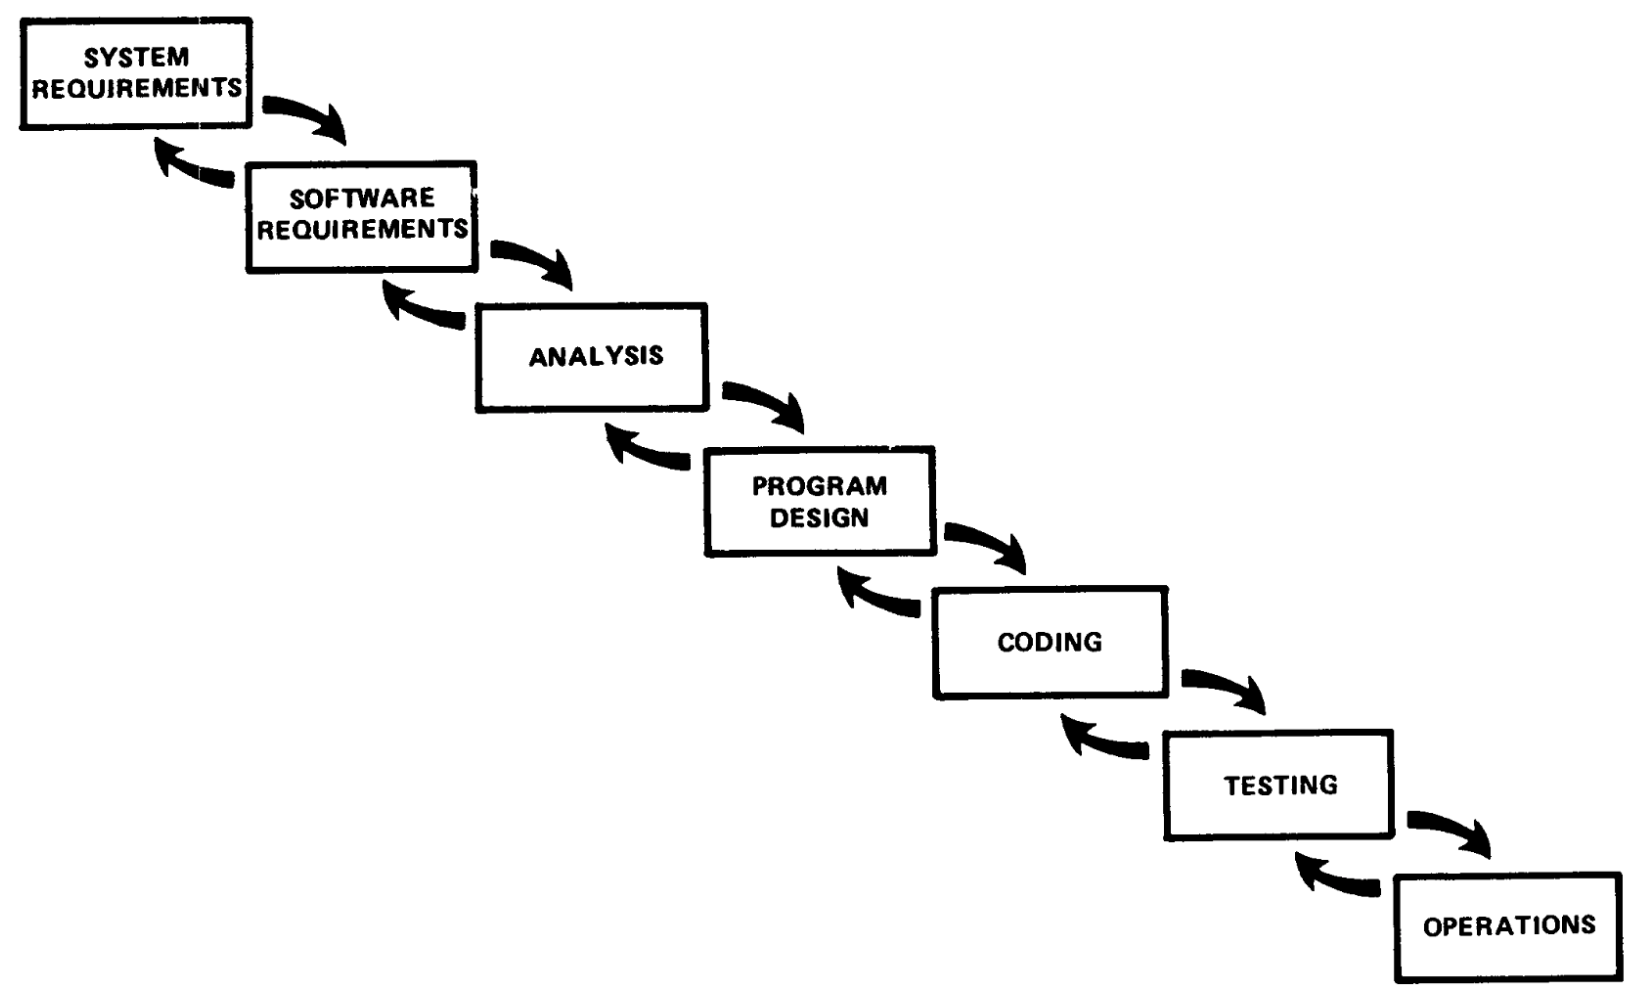
\includegraphics[width=0.9\linewidth]{img/royce-largePrograms}
	\caption{Vorgehensmodell nach Royce}
	\label{img:royce-largePrograms}
\end{figure}


Unsere Bedürfnisse deckt das Vorgehensmodell von Royce ~\cite{Royce1970}, welches in Abbildung  \ref{img:royce-largePrograms} dargestellt ist, am besten ab. Es besteht grundsätzlich aus einem sequentiellen Ablauf der Entwicklungsphasen, berücksichtigt dabei aber auch die Notwendigkeit von Rücksprüngen zur vorherigen Phase.
Die ersten Phasen von der Definition der \textit{System Requirements} bis zu den ersten Gedanken zum Thema \textit{Program Design} behandeln wir im Fachmodul. Der zweite Teil mit der genauen Definition des \textit{Programm Designs} bis zum Betrieb der Software findet anschliessend während der Bachelor-Arbeitszeit statt.


% ################################
% Entwicklungsprozess
% ################################
\subsection{Entwicklungsprozess}
Den Entwicklungsprozess führen wir mit Kanban. Kanban basiert auf dem Pull-Prinzip d.h. jeder, der im Projekt arbeitet, holt sich selbst einen neuen Arbeitsauftrag, sobald er mit einem fertig ist. Die führt dazu, dass die Arbeiten speditiver abgewickelt werden und spart zudem die Stelle des Projektmanagers, der die Aufgaben verteilt.

\begin{figure}[htbp]
	\centering
	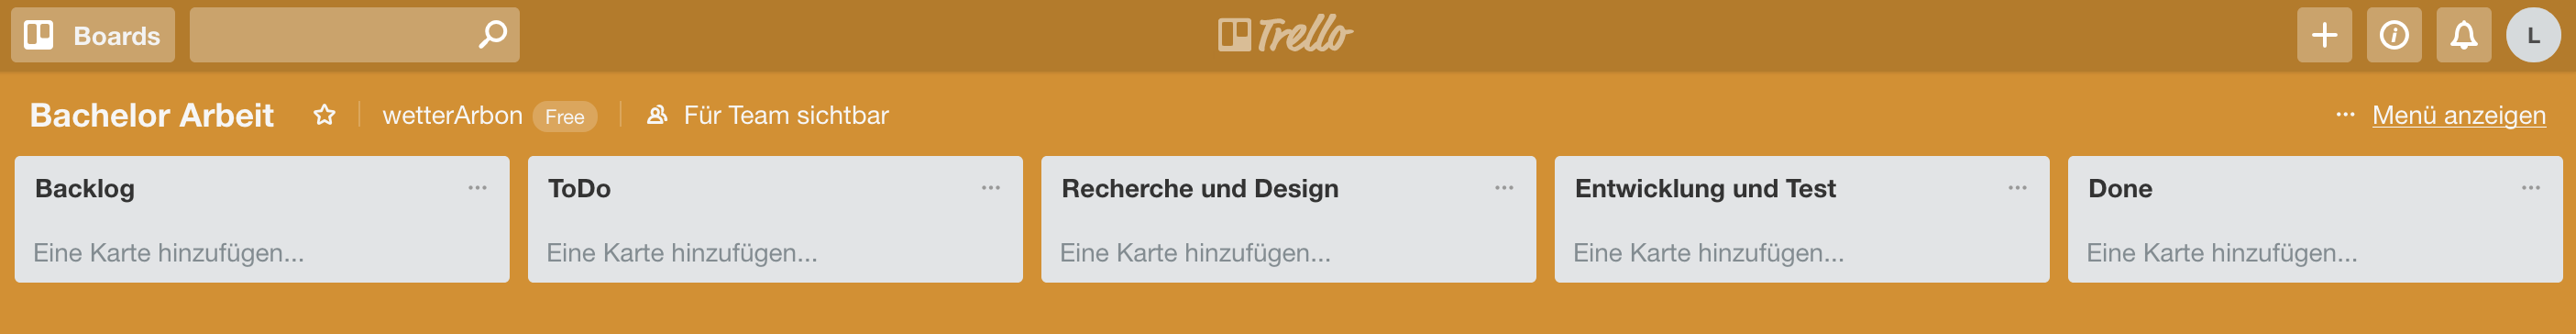
\includegraphics[width=1\linewidth]{img/kanban}
	\caption{Kanban}
	\label{img:kanban}
\end{figure}


David Anderson \cite{AndersonDavidJ2011K:eC} hat das System Kanban, welches ursprünglich aus der Industrie kommt, auf die IT angepasst und dadurch das \textit{Virtuelle Kanban System} entwickelt. Die grundlegenden Regeln daraus lauten:

\begin{itemize}  
\item Jede Karte ist eine Aufgabe
\item Die Aufgabe soll maximal 8 bis16~h benötigen
\item Pro Arbeits-Spalte sind die Anzahl Karten limitiert
\item Eine neue Karte darf erst gezogen werden, wenn die vorherige fertig ist (Multitasking-Vermeidung)
\end{itemize}

% ################################
% Risikoanalyse
% ################################
\subsection{Risikoanalyse}
Für die Risikoanalyse haben wir eine Liste der möglichen  Risiken erstellt. Als Grundlage verwendeten wir das Risikolexikon aus dem Buch \flqq IT-Risikomanagment leben!\frqq ~\cite{AhrendtsFabian2008Il:w}. 
Für jedes Risiko haben wir die Eintretenswahrscheinlichkeit und das Ausmass abgeschätzt. Gegenüber den herkömmlichen Risikobeurteilungen, haben wir allerdings die Auswirkungen auf Kosten und Terminverzug weggelassen, da sie in unserem Projekt nicht relevant sind und uns auf den Stundenaufwand und den Funktionsumfang beschränkt. Um die Auswirkung der einzelen Risiken abschätzen zu können, haben wir eine Punkteskala mit entsprechenden Kriterien erstellt, wie in Tabelle \ref{tab:auswirkung} aufgeführt. \vspace{5mm} %5mm vertical space

\begin{table}[h!]
\centering
\label{tab:auswirkung}
\begin{tabular}{rl}
Wert	[-]	& 	Auswirkung bezüglich Umfang \\
\hline
10	&	Gesamter Block nicht funktionsfähig \\
8	&	Einzelne Funktion nicht umgesetzt  \\
6	&	Bemerkbar, keine Funktionseinbusse \\
4	&	von eingeschränkter Benutzergruppe bemerkbar \\
2	&	von Kunden nicht bemerkbar
\end{tabular}
\end{table}

Die Risikomatrix in Abbildung \ref{img:risikomatrix} zeigt auf grafische Weise wie kritisch die einzelnen Risiken aus der Risikoliste sind. Mindestens vier davon sind als hoch eingestuft und müssen im Rahmen der Bachelor-Arbeit reduziert werden. Dies sind:

\begin{itemize}  
\item Komplexe Datenmigration
\item Mangel an Echtzeitverhalten
\item Mangelnde Ressourcenverfügbarkeit
\item Mangelnde Anforderungsqualität
\end{itemize}


% Abbildung der Risikomatrix
\begin{figure}[h!]
	\centering
	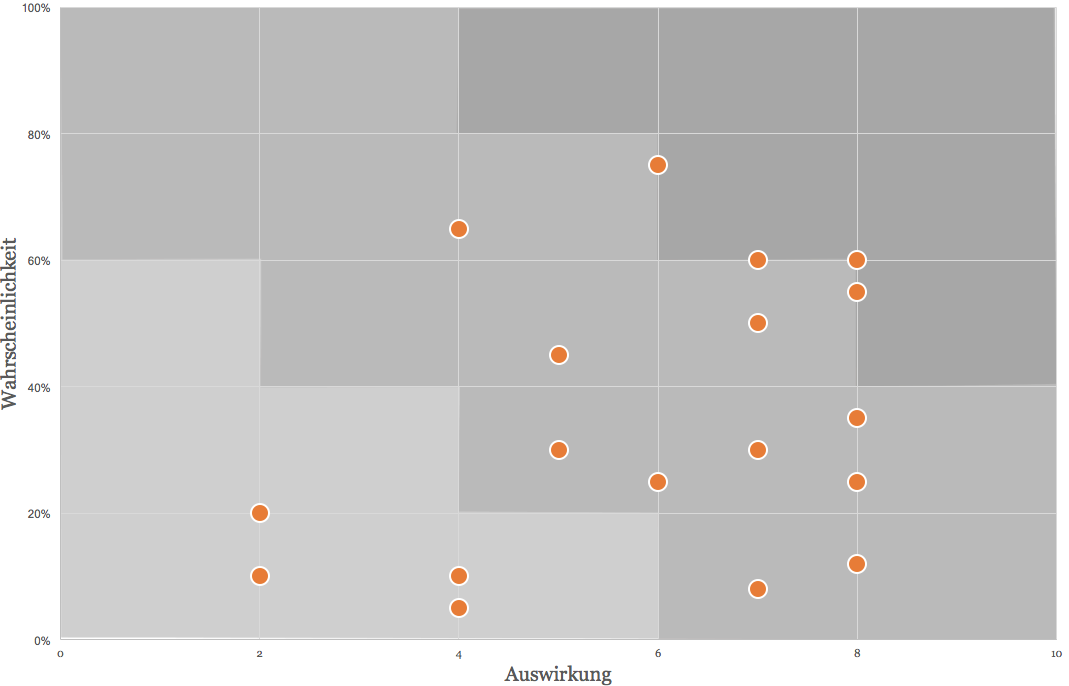
\includegraphics[width=1\linewidth]{img/risikomatrix.pdf} 
	\caption{Risikomatrix}
	\label{img:risikomatrix}
\end{figure}



% ################################
% Projektplan
% ################################

\subsection{Projektplan für die Bachelor-Arbeit}
Der Zeitplan für die Bachelor-Arbeit ist in Abbildung \ref{img:terminplan} auf Seite \pageref{img:terminplan} dargestellt.
Im oberen Teil sind die allgemeinen Termine und Abwesenheiten aufgeführt. Der mittlere Teil zeigt die Arbeitsverteilung über das Semester und am Schluss kommen die Zeitaufwände für Doku und Meetings. Die Dokumentation wollen wir kontinuierlich erstellen, sodass wöchentlich ein entsprechender Block vorgesehen ist.

\begin{figure}[h!]
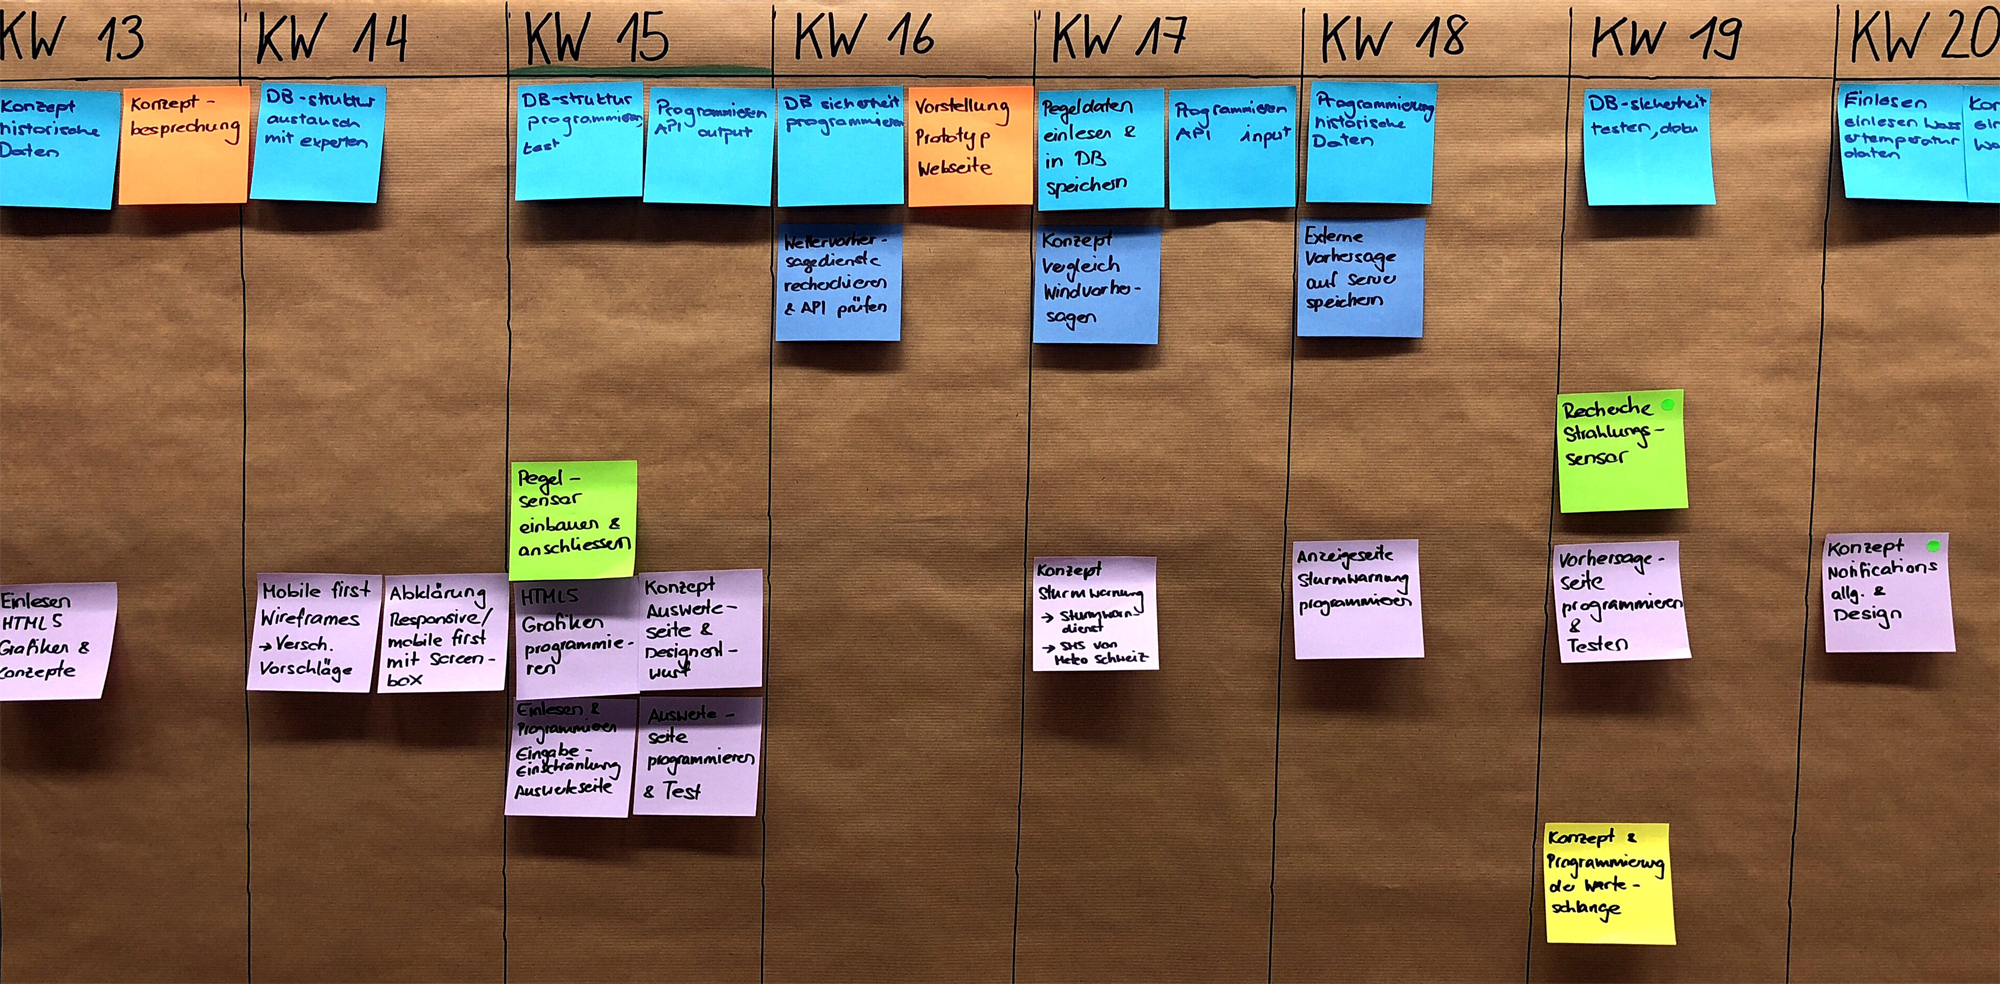
\includegraphics[angle=90,height=1\textheight,keepaspectratio]{img/terminplan.pdf}
\caption{Projektplan für die Bachelor-Arbeit}
\label{img:terminplan}
\end{figure}





% braucht es das?
\FloatBarrier

\subsection{Dokumentation}

%Allgemein
Für die Bachelor-Arbeit verwenden wir unterschiedliche Dokumentationswerkzeuge. Bei der Auswahl haben wir darauf geachtet, das die Tools kostenlos nutzbar und für sämtliche Plattformen verfügbar sind (Windows, Mac, iPad, usw.). Weiter war uns wichtig, dass die Tools untereinander kommunizieren können. 

% github / Trello / Toggl
\subsubsection*{Versionierung und Zeiterfassung}
Sämtliche Artefakte speichern wir auf \textit{github}. Wir haben somit eine automatische Versionierung der Dokumente und können unabhängig voneinander an den Dokumenten arbeiten. Die Planung bzw. Darstellung des Entwicklungsprozesses erledigen wir mir \textit{Trello}. Es ist eine intuitive Webanwendung, welche diverse Integrationsmöglichkeiten mit den anderen Tools bietet. Für die Zeiterfassung verwenden wir \textit{Toggl}, welches mittels Plugin direkt in Trello integriert werden kann.

% Kommunikation nach aussen
\subsubsection*{Reporting; Kommunikation extern}
Damit wir keine Besprechungsprotokolle verschicken müssen und alle Informationen für alle immer zugänglich sind, haben wir entschieden, das Reporting in Form einer öffentlichen Webseite zu erstellen. github bietet mit \textit{GitPages} einen Hosting-Service an, der genau dies ermöglicht. Der Vorteil von \textit{GitPages} ist, dass wir sämtliche Daten in einem einzigen Ort bzw. Repository vereint haben. Damit wir uns nicht mit Formatierung herumschlagen müssen und uns auf den Inhalt konzentrieren können, verwenden wir \textit{mkdocs} als Template Engine. Die Webseiten-Einträge können wir dadurch auf simple Art in Form von Markdown-Files erstellen.

% Kommunikation nach innen
\subsubsection*{Kommunikation teamintern}
Innerhalb des Teams nutzen wir das Kommunikationstool \textit{Slack}. Dieses ermöglicht uns, Konversationen als Chat aufzuzeichnen und nach Themen zu gruppieren. Weiter lassen sich Dokumente austauschen. Sämtliche git-Posts werden von Slack automatisch geloggt und können, falls gewünscht, als push-Notification angezeigt werden.
Das wöchentliche Team-Meeting findet über \textit{Skype} statt, da wir den regelmässigen mündlichen Austausch als zentralen Punkt erachten.

% Bericht = LaTeX
\subsubsection*{Dokumentation}
Den Bericht werden wir in \LaTeX\ verfassen. Wir haben uns für \LaTeX\ entschieden, da wir uns auf den Inhalt konzentrieren können und das Layout automatisiert ist. Weiter ist \LaTeX\ in der Wissenschaft weit verbreitet. Die Bachelor-Arbeit ist deshalb eine gute Gelegenheit, uns in dieses Thema einzuarbeiten.




\subsection{Risikoliste}
Ausgearbeitet mit dem Risikolexikon aus dem Buch xxxx, Risikoschablone
siehe ~\cite{AhrendtsFabian2008Il:w}.


\subsection{Risikoanalyse und Risikomatrix}





   
\section{Rechtliche Ansprüche}
siehe separates Dokument
%%%%%%%%%%%%%%%%%%%%%%%%%%%%%%%%%%%
%%  Schluss
%%%%%%%%%%%%%%%%%%%%%%%%%%%%%%%%%%%
\section{Schluss}
% viele Konzepte
Während der Analyse der Wetterstation konnten wir diverse Schwachstellen ausfindig machen, die mehr oder weniger dringend beseitigt werden müssen.
Bei vielen Problemen muss zuerst ein Lösungskonzept erstellt werden, bevor mit der Behebung begonnen werden kann. Diese Arbeit bedarf einiges an Recherchearbeit und darf nicht unterschätzt werden.
\newline

\noindent
% unbekannte Thematik
Das gesamte Themengebiet von Barrierefreiheit und User Interface Design ist für uns neu und wir müssen das gesamt Know-how von Grund auf aufbauen. Ebenso ist die Arbeit mit Skripten und die Verdünnung der Daten auf einer Datenbank neu für uns. Auch hier ist ein grosser Teil für Einlesearbeiten zu erwarten.
\newline

\noindent
% schwierige Rahmenbedingungen
Als kritisch bezwiehungsweise schwer abschätzbar sehen wir die gegebenen Rahmenbedingung, die uns allenfalls in der Lösungsfindung stark einschränken.
Zum Beispiel ist dies das vorgegebene CMS oder die Schnittstelle zum Kombi-Wetter-Transmitter über \textit{WeatherDisplay}.
\newline

\noindent
% Rückblick auf Stundenschätzung
Anfangs Fachmodul schätzen wir die Stundenaufwände für die während dem Fachmodul anstehenden Arbeiten ab. Die effektiven Aufwände haben wir mittels Toggl dokumentier, sodass wir nun am Schluss des Fachmoduls die geleisteten Stunden den geplanten gegenüberstellen können. Die Auflistung befindet sich in Tabelle~\ref{plan-ist}. 
Sowohl die produktiven Arbeiten, d.h. die Arbeiten, die gemäss Fachmodul-Auftrag zu erledigen waren, als auch die Administrativen Aufwände für Meetings und Wochenreports stimmen recht gut. Der Aufwand für die Dokumentation hingegen haben wir unterschätzt. Wenn wir anfangs Bachelor-Arbeit den definitiven Terminplan erstellen müssen wir dies berücksichtigen.
\newline

\begin{table}[h]
\centering
\begin{tabular}{|l|l|l|l|}
\hline
 Tätigkeit			&  Plan	& Ist  	& Delta  		\\ \hline
 Produktive Arbeit	&  86		&  75		&  13~\%		\\ \hline
 Dokumentation		&  44		&  73		&  65~\%		\\ \hline
 Administration		&  30		&  27		&  10~\%		\\ \hline
\end{tabular}
\caption{Vergleich der Planstunden zu den Ist-Stunden}
\label{table:plan-ist}
\end{table}

\noindent
Zusammenfassend sehen wir Bachelor-Arbeit als machbar an. Zeitlich bleibt jedoch nicht viel Spielraum. Die grossen Unbekannten wie  einschränkende Rahmenbedingungen und schwer abzuschätzenden Aufwand für Einarbeitung und Konzepterstellung bedingen jedoch, dass der Fortschritt kontinuierlich und kritisch geprüft wird.


\bibliography{literatur}{}	
\bibliographystyle{plain}

\end{document}
